\documentclass[10pt,a4paper]{article}
\usepackage[margin=18mm,top=20mm,bottom=18mm]{geometry}
\usepackage{fontspec,graphicx,amsmath,booktabs,xcolor,fancyhdr}
\setmainfont{DejaVu Sans}
\newfontfamily\jpfont[Path=/usr/share/fonts/google-droid-sans-fonts/,BoldFont=DroidSansFallbackFull.ttf,BoldFeatures={FakeBold=1.2}]{DroidSansFallbackFull.ttf}
\XeTeXlinebreaklocale "ja"
\XeTeXlinebreakskip=0pt plus 1pt
\definecolor{navy}{HTML}{17385D}
\pagestyle{fancy}\fancyhf{}\fancyhead[L]{\small STAR / Nuclear PID and Purity}\fancyhead[R]{\small Gaussian + linear}\fancyfoot[C]{\thepage}\setlength{\headheight}{14pt}
\emergencystretch=2em\setlength{\parindent}{0pt}\setlength{\parskip}{5pt}\linespread{1.10}
\begin{document}
\section*{\hspace{0pt}{\jpfont 原子核}\hspace{0pt}PID\hspace{0pt}{\jpfont と}\hspace{0pt}Purity\hspace{0pt}{\jpfont 推定}\hspace{0pt}}
Gaussian\hspace{0pt}{\jpfont 応答＋}\hspace{0pt}linear\hspace{0pt}{\jpfont 背景による最終表示}\hspace{0pt} /\allowbreak{} 2026\hspace{0pt}{\jpfont 年}\hspace{0pt}10\hspace{0pt}{\jpfont 月}\hspace{0pt}21\hspace{0pt}{\jpfont 日}\hspace{0pt}

\hspace{0pt}{\jpfont 対象：}\hspace{0pt}2021 P24iy\hspace{0pt}{\jpfont 、}\hspace{0pt}auau3p85\hspace{0pt}{\jpfont 解析試料。}\hspace{0pt}d\hspace{0pt}{\jpfont 、}\hspace{0pt}t\hspace{0pt}{\jpfont 、}\hspace{0pt}³He\hspace{0pt}{\jpfont 、}\hspace{0pt}⁴He\hspace{0pt}{\jpfont について、}\hspace{0pt}R=|p/\allowbreak{}q|\hspace{0pt}{\jpfont ごとの}\hspace{0pt}Purity\hspace{0pt}{\jpfont を推定する。}\hspace{0pt}R<2 GeV/\allowbreak{}c\hspace{0pt}{\jpfont は}\hspace{0pt}TOF\hspace{0pt}{\jpfont を使わない}\hspace{0pt}ALL\hspace{0pt}{\jpfont 、}\hspace{0pt}R≥2 GeV/\allowbreak{}c\hspace{0pt}{\jpfont は既存}\hspace{0pt}TOF m²\hspace{0pt}{\jpfont 選択を用いる。}\hspace{0pt}

\hspace{0pt}{\jpfont 目視判断とユーザー指定に従い、全核種を}\hspace{0pt}Gaussian\hspace{0pt}{\jpfont ＋}\hspace{0pt}linear\hspace{0pt}{\jpfont の名目}\hspace{0pt}fit\hspace{0pt}{\jpfont だけに統一した。背景なし・}\hspace{0pt}lognormal\hspace{0pt}{\jpfont ・}\hspace{0pt}exponential\hspace{0pt}{\jpfont の点、他モデル由来の範囲はこの}\hspace{0pt}Purity\hspace{0pt}{\jpfont 図に含めない。}\hspace{0pt}

\begin{center}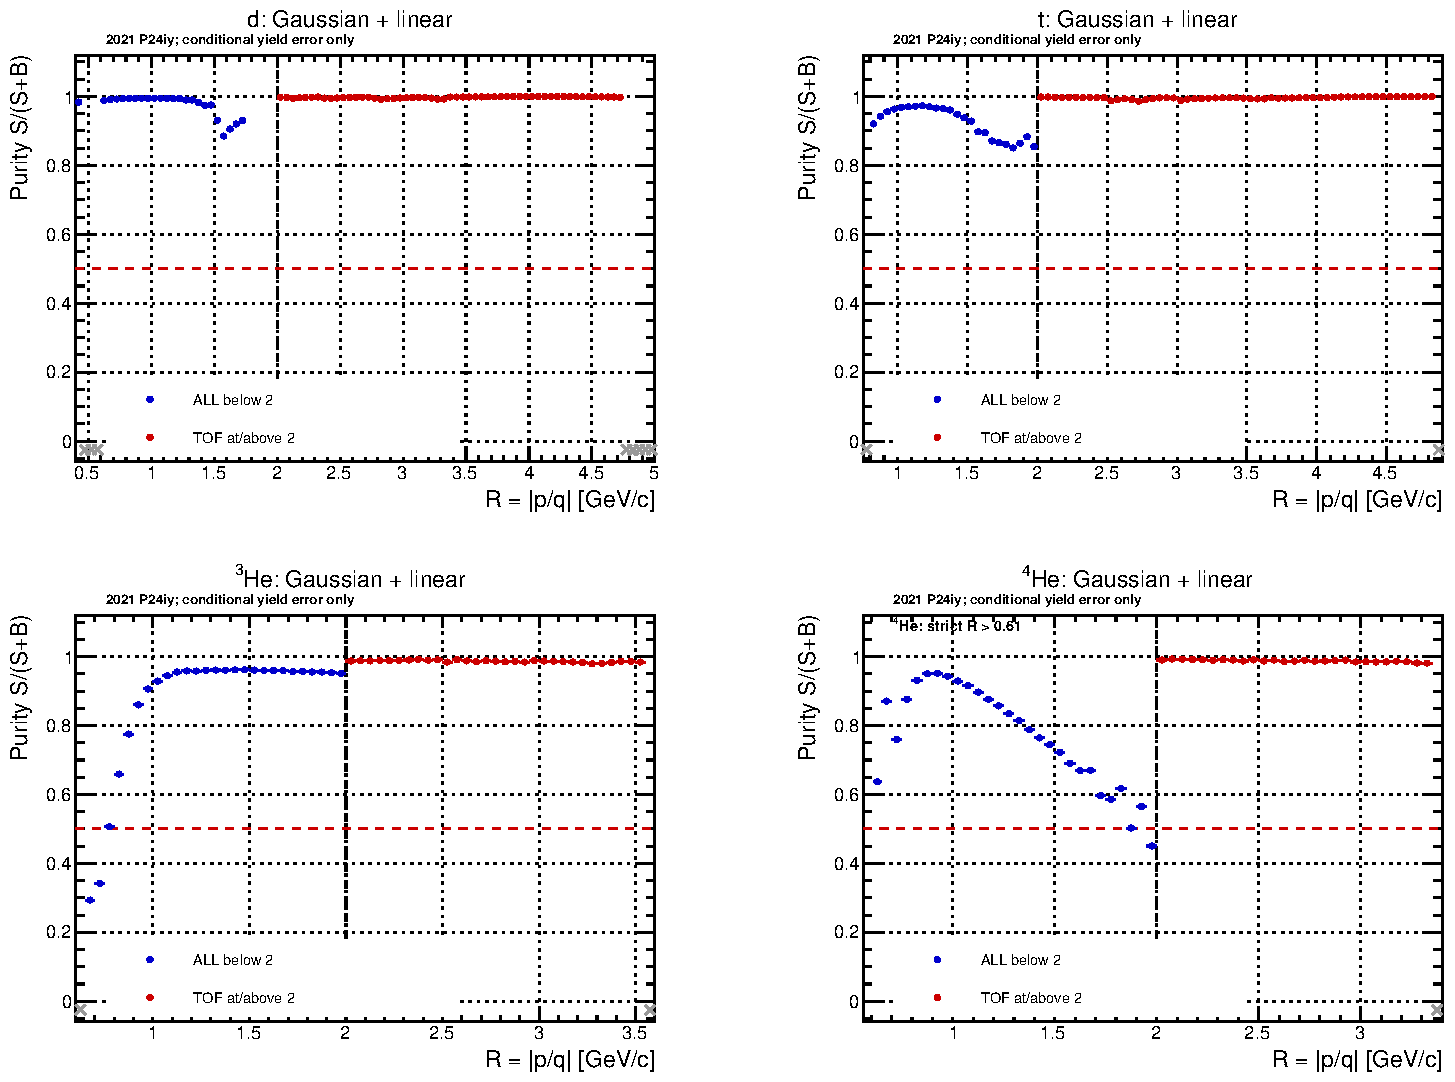
\includegraphics[width=\linewidth,height=.57\textheight,keepaspectratio]{purity_vs_p_over_q_01_trim.png}\end{center}
\hspace{0pt}{\jpfont 図}\hspace{0pt}1\hspace{0pt}{\jpfont 　更新した最終}\hspace{0pt}Purity\hspace{0pt}{\jpfont 。青：}\hspace{0pt}ALL\hspace{0pt}{\jpfont 、赤：}\hspace{0pt}TOF\hspace{0pt}{\jpfont 。横誤差は}\hspace{0pt}R\hspace{0pt}{\jpfont 区間、縦誤差は収量の条件付き誤差。灰色の}\hspace{0pt}×\hspace{0pt}{\jpfont は}\hspace{0pt}Gaussian\hspace{0pt}{\jpfont ＋}\hspace{0pt}linear\hspace{0pt}{\jpfont 自身の支持条件を通らない区間。}\hspace{0pt}

⁴He\hspace{0pt}{\jpfont は}\hspace{0pt}R>0.61\hspace{0pt}{\jpfont を適用。}\hspace{0pt}0.61–0.65\hspace{0pt}{\jpfont の}\hspace{0pt}Purity\hspace{0pt}{\jpfont は}\hspace{0pt}63.70 ± 0.07\%\hspace{0pt}{\jpfont （条件付き誤差）。本報告は解析候補の更新をまとめたもので、本番設定への反映は行っていない。}\hspace{0pt}


\clearpage
\section*{1. \hspace{0pt}{\jpfont 選別と}\hspace{0pt}Purity\hspace{0pt}{\jpfont の定義}\hspace{0pt}}
R\hspace{0pt}{\jpfont は電荷で割った運動量であり、電荷}\hspace{0pt}2\hspace{0pt}{\jpfont の}\hspace{0pt}He\hspace{0pt}{\jpfont では運動量そのものと異なる。}\hspace{0pt}TPC\hspace{0pt}{\jpfont の}\hspace{0pt}dE/\allowbreak{}dx PID\hspace{0pt}{\jpfont は中心}\hspace{0pt}μPID(R)\hspace{0pt}{\jpfont と幅}\hspace{0pt}σPID(R)\hspace{0pt}{\jpfont で定義し、厳密な}\hspace{0pt}|nσ|<2\hspace{0pt}{\jpfont と}\hspace{0pt}best-species\hspace{0pt}{\jpfont 判定を用いる。重複時は}\hspace{0pt}|nσ|\hspace{0pt}{\jpfont が最小の核種を採用し、同値の優先順は}\hspace{0pt}d\hspace{0pt}{\jpfont 、}\hspace{0pt}t\hspace{0pt}{\jpfont 、}\hspace{0pt}³He\hspace{0pt}{\jpfont 、}\hspace{0pt}⁴He\hspace{0pt}{\jpfont 。}\hspace{0pt}

\[n\sigma_i(R,x)=\frac{x-\mu_{\mathrm{PID},i}(R)}{\sigma_{\mathrm{PID},i}(R)},\qquad |n\sigma_i|<2.\]
\hspace{0pt}{\jpfont 観測スペクトルは}\hspace{0pt}d\hspace{0pt}{\jpfont 、}\hspace{0pt}t\hspace{0pt}{\jpfont 、}\hspace{0pt}³He\hspace{0pt}{\jpfont 、}\hspace{0pt}⁴He\hspace{0pt}{\jpfont の}\hspace{0pt}Gaussian\hspace{0pt}{\jpfont 成分と}\hspace{0pt}linear\hspace{0pt}{\jpfont な}\hspace{0pt}smooth\hspace{0pt}{\jpfont 背景の和で}\hspace{0pt}fit\hspace{0pt}{\jpfont する。}\hspace{0pt}linear\hspace{0pt}{\jpfont 背景は}\hspace{0pt}fit\hspace{0pt}{\jpfont 領域内で非負になる端点基底を用いる。右側の}\hspace{0pt}log\hspace{0pt}{\jpfont 表示は縦軸の表示方法であり、}\hspace{0pt}lognormal\hspace{0pt}{\jpfont 応答を採用したものではない。}\hspace{0pt}

\[f(x;R)=\sum_{i=d,t,{}^3\mathrm{He},{}^4\mathrm{He}}N_i(R)G_i(x;\mu_i,s_i)+B_{\rm linear}(x;R).\]
\hspace{0pt}{\jpfont 核種}\hspace{0pt}i\hspace{0pt}{\jpfont の}\hspace{0pt}PID\hspace{0pt}{\jpfont 選択領域へ各成分を積分し、}\hspace{0pt}S\hspace{0pt}{\jpfont を目的核種、}\hspace{0pt}B\hspace{0pt}{\jpfont を他核種の混入と}\hspace{0pt}linear\hspace{0pt}{\jpfont 背景の和とする。複数}\hspace{0pt}native\hspace{0pt}{\jpfont 区間をまとめる際は}\hspace{0pt}Purity\hspace{0pt}{\jpfont の平均ではなく、分子・分母を先に合計する。}\hspace{0pt}

\[P_i=\frac{S_i}{S_i+B_i},\qquad P_i(\Delta R)=\frac{\sum_k S_{i,k}}{\sum_k (S_{i,k}+B_{i,k})}.\]
\begin{center}\small\begin{tabular}{lr}\toprule
R\hspace{0pt}{\jpfont 領域}\hspace{0pt} & \hspace{0pt}{\jpfont 試料・条件}\hspace{0pt}\\\midrule
{}R<2 & ALL\hspace{0pt}{\jpfont ：}\hspace{0pt}TOF\hspace{0pt}{\jpfont による試料選択なし}\hspace{0pt}\\
{}R≥2 & \hspace{0pt}{\jpfont 既存の核種別}\hspace{0pt}TOF m²\hspace{0pt}{\jpfont 窓}\hspace{0pt}\\
{}⁴He\hspace{0pt}{\jpfont 全域}\hspace{0pt} & strict R>0.61\hspace{0pt}{\jpfont 、}\hspace{0pt}TOF\hspace{0pt}{\jpfont 側は}\hspace{0pt}d\hspace{0pt}{\jpfont と同じ}\hspace{0pt}m²\hspace{0pt}{\jpfont 窓}\hspace{0pt}\\\bottomrule\end{tabular}\end{center}
\begin{center}\small\begin{tabular}{lrr}\toprule
\hspace{0pt}{\jpfont 核種}\hspace{0pt} & TOF m²\hspace{0pt}{\jpfont 下限}\hspace{0pt} & TOF m²\hspace{0pt}{\jpfont 上限}\hspace{0pt}\\\midrule
{}d & 3.268773 & 3.693147\\
{}t & 7.256428 & 8.281693\\
{}he3 & 1.78285 & 2.06485\\
{}he4 & 3.268773 & 3.693147\\\bottomrule\end{tabular}\end{center}
\hspace{0pt}{\jpfont 通常の表示は}\hspace{0pt}0.05 GeV/\allowbreak{}c\hspace{0pt}{\jpfont 幅。低}\hspace{0pt}R\hspace{0pt}{\jpfont の}\hspace{0pt}native\hspace{0pt}{\jpfont 幅は}\hspace{0pt}0.01\hspace{0pt}{\jpfont 。}\hspace{0pt}⁴He\hspace{0pt}{\jpfont の最初の集約区間のみ下限で}\hspace{0pt}clip\hspace{0pt}{\jpfont し、}\hspace{0pt}0.61–0.65\hspace{0pt}{\jpfont の}\hspace{0pt}4 native\hspace{0pt}{\jpfont 区間を使う。}\hspace{0pt}TOF\hspace{0pt}{\jpfont 側}\hspace{0pt}⁴He\hspace{0pt}{\jpfont は既存の}\hspace{0pt}0.05\hspace{0pt}{\jpfont 幅}\hspace{0pt}fit\hspace{0pt}{\jpfont を維持する。}\hspace{0pt}R\hspace{0pt}{\jpfont 方向は}\hspace{0pt}GL3\hspace{0pt}{\jpfont で積分し、選択窓の生計数は}\hspace{0pt}native dE/\allowbreak{}dx bin\hspace{0pt}{\jpfont との重なり比で評価する。イベント単位の}\hspace{0pt}PID\hspace{0pt}{\jpfont 再選択ではない。}\hspace{0pt}


\clearpage
\section*{2. PID\hspace{0pt}{\jpfont 関数形と係数の更新}\hspace{0pt}}
Git 8f7d539\hspace{0pt}{\jpfont の元の関数形へ戻り、}\hspace{0pt}x=log10 R\hspace{0pt}{\jpfont に対する中心}\hspace{0pt}3\hspace{0pt}{\jpfont 次・幅}\hspace{0pt}2\hspace{0pt}{\jpfont 次を維持した。}\hspace{0pt}d/\allowbreak{}t\hspace{0pt}{\jpfont の係数は不変更。}\hspace{0pt}He\hspace{0pt}{\jpfont の係数のみ既存}\hspace{0pt}ALL\hspace{0pt}{\jpfont ・}\hspace{0pt}TOF\hspace{0pt}{\jpfont の自由}\hspace{0pt}fit\hspace{0pt}{\jpfont 参照に基づき微調整した。}\hspace{0pt}

\begin{align*}x&=\log_{10}\!\left(R/(1\,{\rm GeV}/c)\right),\\ \mu_{\rm PID}(R)&=a_0+a_1x+a_2x^2+a_3x^3,\\ \sigma_{\rm PID}(R)&=b_0+b_1x+b_2x^2.\end{align*}
\begin{center}\small\begin{tabular}{lrrrr}\toprule
\hspace{0pt}{\jpfont 核種}\hspace{0pt} & a0 & a1 & a2 & a3\\\midrule
{}d & 10.2875 & -36.6639 & 67.63 & -45.2483\\
{}t & 19.2177 & -70.3198 & 113.876 & -67.0591\\
{}³He & 28.9366924 & -70.3530693 & 110.508931 & -63.6022153\\
{}⁴He & 40.0445053 & -103.726 & 138.340359 & -63.6019056\\\bottomrule\end{tabular}\end{center}
\begin{center}\small\begin{tabular}{lrrr}\toprule
\hspace{0pt}{\jpfont 核種}\hspace{0pt} & b0 & b1 & b2\\\midrule
{}d & 0.771189 & -2.63609 & 2.8044\\
{}t & 1.40996 & -4.97147 & 4.97608\\
{}³He & 1.59382851 & -3.93029659 & 3.57884443\\
{}⁴He & 2.21905518 & -7.21800964 & 8.81443825\\\bottomrule\end{tabular}\end{center}
\hspace{0pt}{\jpfont 係数の調整では中心変化を元の}\hspace{0pt}σ\hspace{0pt}{\jpfont の}\hspace{0pt}0.5\hspace{0pt}{\jpfont 倍以内、幅変化を元の}\hspace{0pt}σ\hspace{0pt}{\jpfont の}\hspace{0pt}20\%\hspace{0pt}{\jpfont 以内とし、}\hspace{0pt}R=0.4–5\hspace{0pt}{\jpfont の監査域で中心と幅の正値を検証した。表は丸めた表示であり、再現には同梱}\hspace{0pt}coefficients.json\hspace{0pt}{\jpfont の全桁を用いる。}\hspace{0pt}

\hspace{0pt}{\jpfont 重要な区別：この}\hspace{0pt}μPID\hspace{0pt}{\jpfont 、}\hspace{0pt}σPID\hspace{0pt}{\jpfont は選択窓の関数であり、各}\hspace{0pt}1\hspace{0pt}{\jpfont 次元スペクトル}\hspace{0pt}fit\hspace{0pt}{\jpfont の}\hspace{0pt}Gaussian\hspace{0pt}{\jpfont 中心}\hspace{0pt}μfit\hspace{0pt}{\jpfont 、幅}\hspace{0pt}sfit\hspace{0pt}{\jpfont と同一ではない。後述の低}\hspace{0pt}R\hspace{0pt}{\jpfont ピーク修正は}\hspace{0pt}fit\hspace{0pt}{\jpfont の参照成分に反映しており、}\hspace{0pt}TPC PID\hspace{0pt}{\jpfont の多項式を局所補間へ置き換えていない。}\hspace{0pt}

\hspace{0pt}{\jpfont 今回追加した選択条件は}\hspace{0pt}⁴He\hspace{0pt}{\jpfont の}\hspace{0pt}R>0.61\hspace{0pt}{\jpfont 。多項式の中心・幅の係数は直前の候補から維持した。}\hspace{0pt}³He\hspace{0pt}{\jpfont の選択関数を、}\hspace{0pt}⁴He fit\hspace{0pt}{\jpfont 内の}\hspace{0pt}³He\hspace{0pt}{\jpfont 参照中心と混同しない。}\hspace{0pt}

\hspace{0pt}{\jpfont 本番}\hspace{0pt}PID\hspace{0pt}{\jpfont 設定は未変更。解析候補の選択条件、係数元と低}\hspace{0pt}R\hspace{0pt}{\jpfont 応答較正を}\hspace{0pt}pid\_\allowbreak{}selection.yaml\hspace{0pt}{\jpfont に分けて保存している。}\hspace{0pt}


\clearpage
\section*{3. PID\hspace{0pt}{\jpfont 中心の変更前後}\hspace{0pt}}
\begin{center}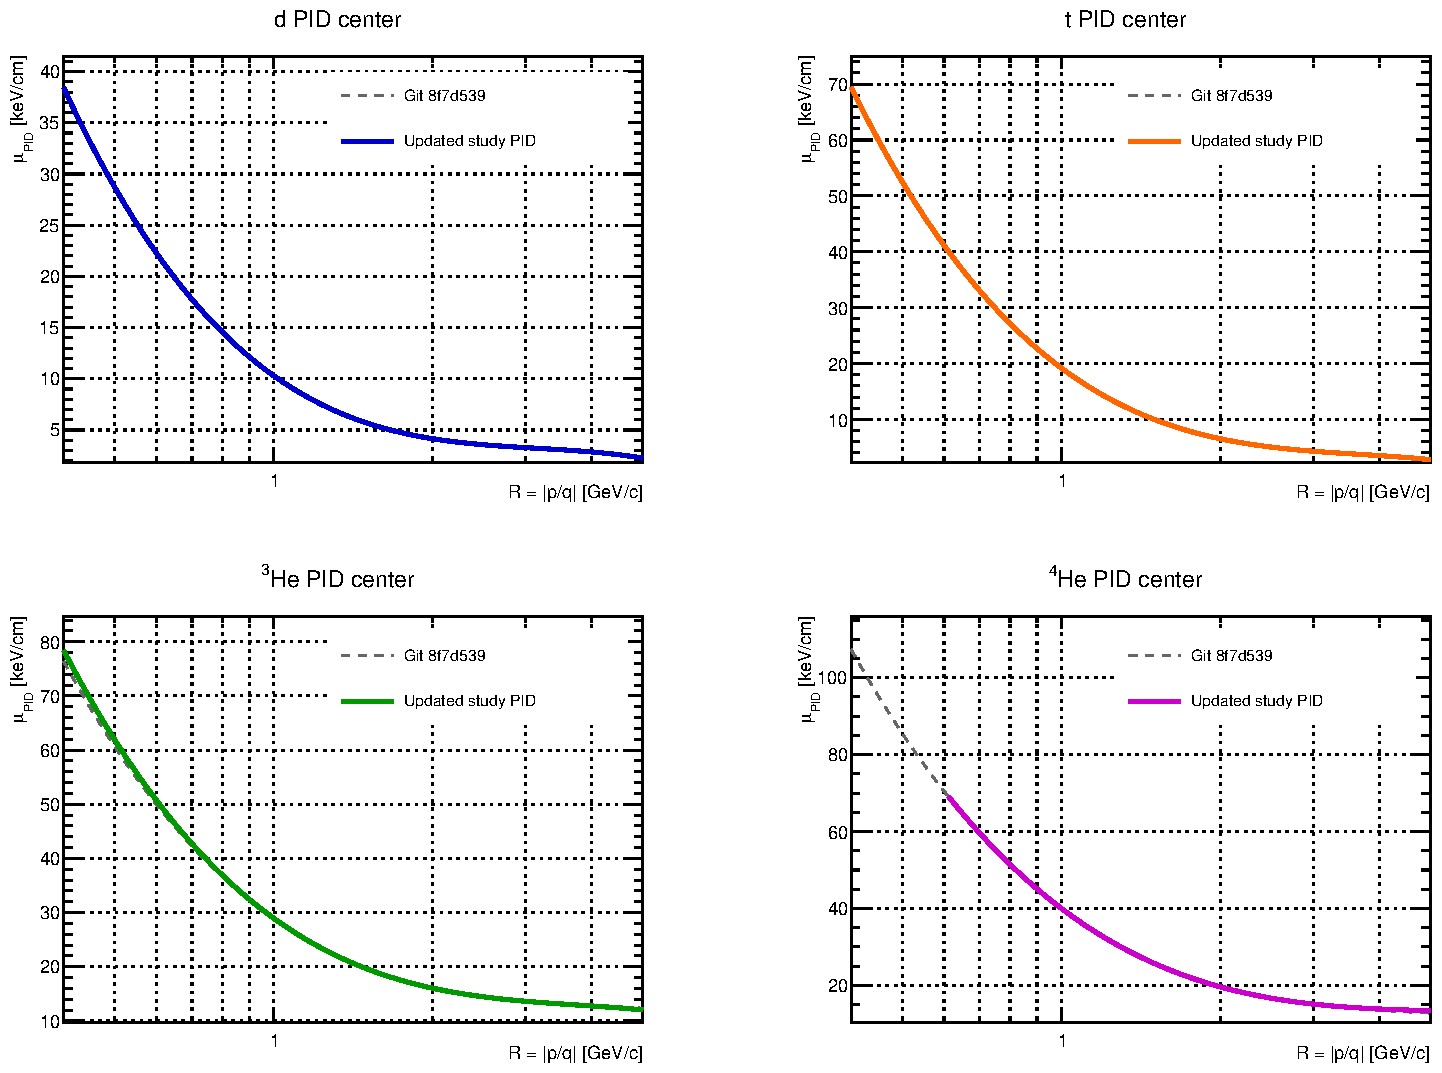
\includegraphics[width=\linewidth,height=.72\textheight,keepaspectratio]{pid_function_updates_01_trim.png}\end{center}
\hspace{0pt}{\jpfont 図}\hspace{0pt}2\hspace{0pt}{\jpfont 　元の}\hspace{0pt}Git\hspace{0pt}{\jpfont 関数（灰色破線）と解析候補（色線）の中心}\hspace{0pt}μPID\hspace{0pt}{\jpfont 。}\hspace{0pt}d/\allowbreak{}t\hspace{0pt}{\jpfont は重なる。}\hspace{0pt}He\hspace{0pt}{\jpfont は従来の}\hspace{0pt}3\hspace{0pt}{\jpfont 次式の係数だけを微調整した。}\hspace{0pt}⁴He\hspace{0pt}{\jpfont の候補曲線は適用範囲}\hspace{0pt}R>0.61\hspace{0pt}{\jpfont に限定して表示した。}\hspace{0pt}

\hspace{0pt}{\jpfont この図は}\hspace{0pt}PID\hspace{0pt}{\jpfont 選択窓の中心であり、低}\hspace{0pt}R Gaussian fit\hspace{0pt}{\jpfont の中心を示す図ではない。指定された}\hspace{0pt}R=0.61/\allowbreak{}0.64\hspace{0pt}{\jpfont のピーク位置は後述の応答較正へ反映する。}\hspace{0pt}


\clearpage
\section*{4. PID\hspace{0pt}{\jpfont 幅の変更前後}\hspace{0pt}}
\begin{center}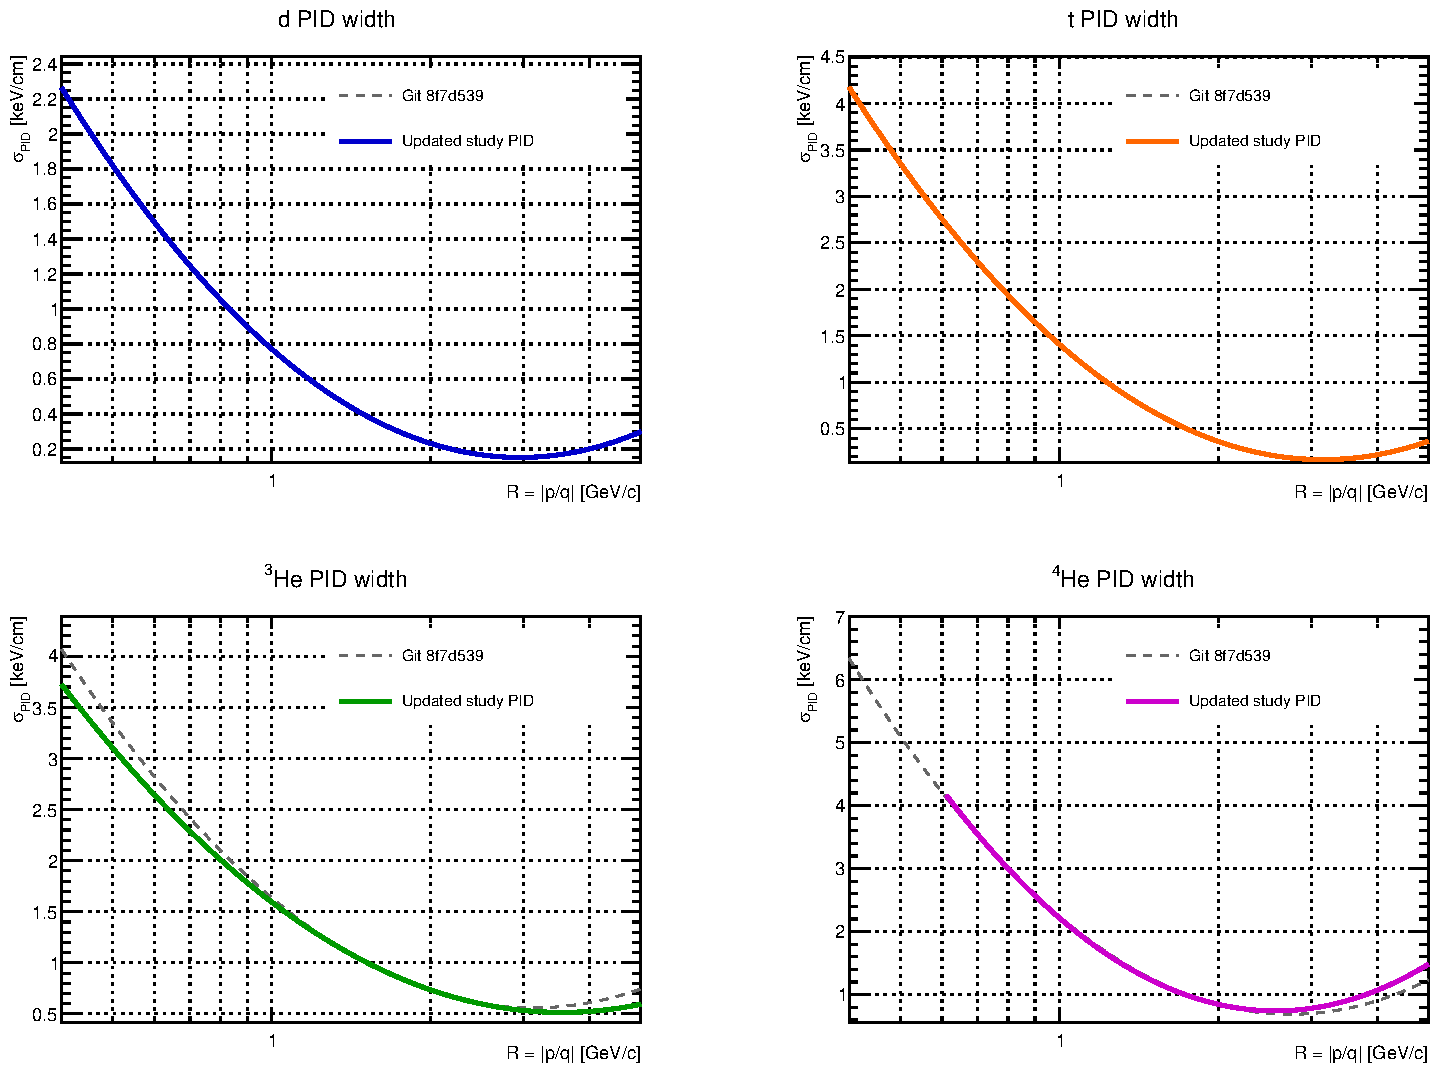
\includegraphics[width=\linewidth,height=.72\textheight,keepaspectratio]{pid_function_updates_02_trim.png}\end{center}
\hspace{0pt}{\jpfont 図}\hspace{0pt}3\hspace{0pt}{\jpfont 　元の}\hspace{0pt}Git\hspace{0pt}{\jpfont 関数と候補の幅}\hspace{0pt}σPID\hspace{0pt}{\jpfont 。幅は}\hspace{0pt}log10 R\hspace{0pt}{\jpfont の}\hspace{0pt}2\hspace{0pt}{\jpfont 次式であり、新しいガタガタした補間は導入していない。幅の正値と変更量を監査した。}\hspace{0pt}

\hspace{0pt}{\jpfont 選択窓は}\hspace{0pt}μPID±2σPID\hspace{0pt}{\jpfont に加え、核種間の}\hspace{0pt}best-species\hspace{0pt}{\jpfont 判定で区切られる。したがって、図の帯を単独で切り取っただけの選択ではない。}\hspace{0pt}


\clearpage
\section*{5. dE/\allowbreak{}dx\hspace{0pt}{\jpfont 分布と選択曲線}\hspace{0pt}}
\begin{center}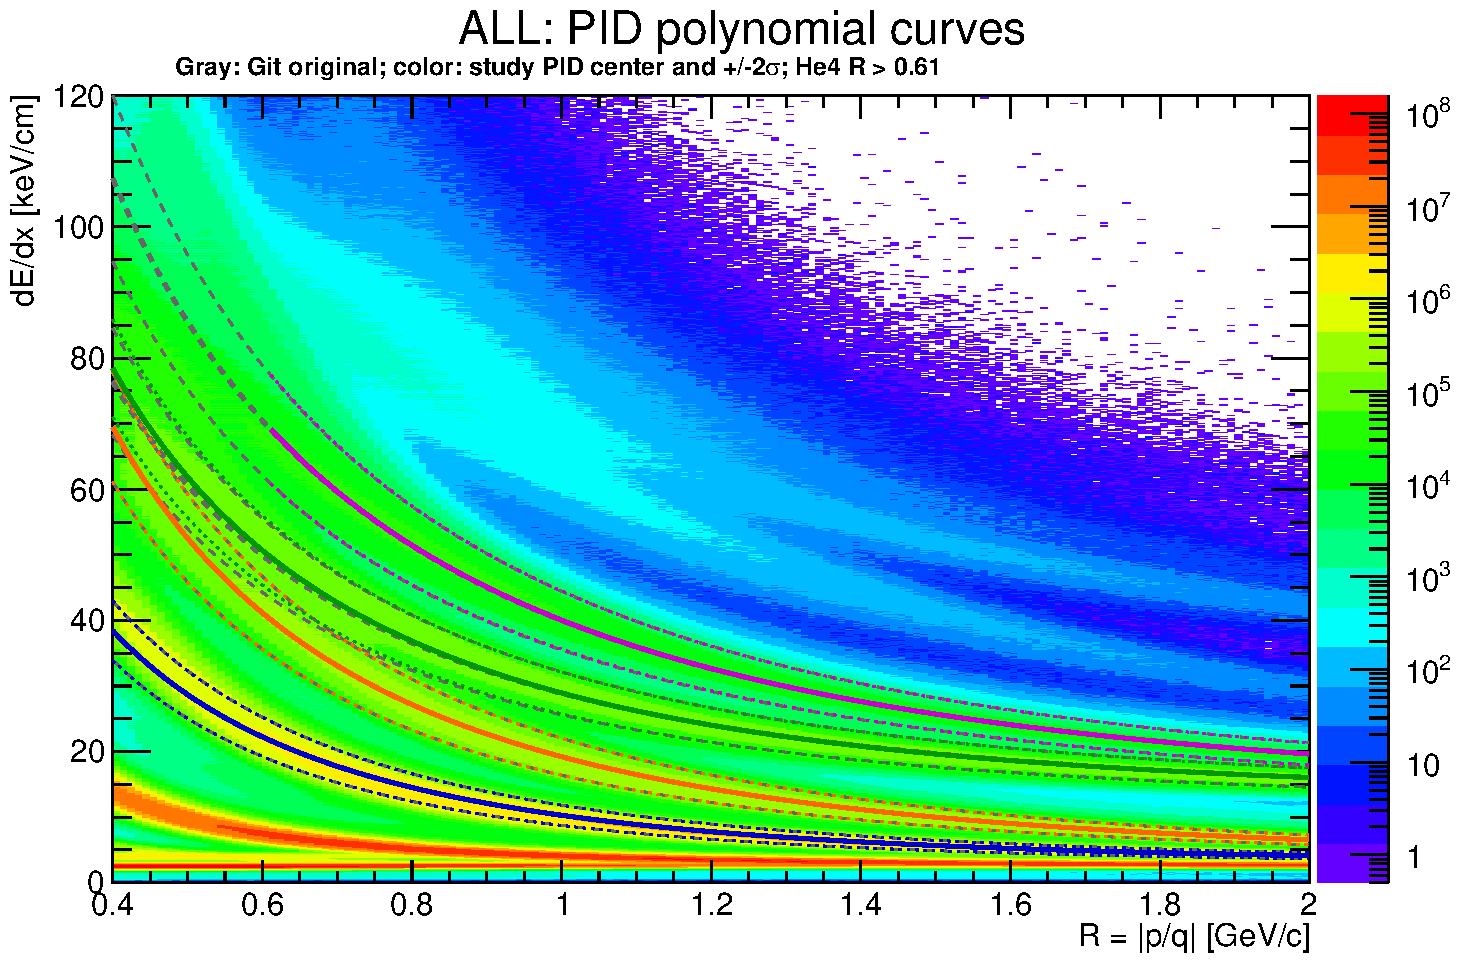
\includegraphics[width=\linewidth,height=.61\textheight,keepaspectratio]{dedx_pid_map_01_trim.png}\end{center}
\hspace{0pt}{\jpfont 図}\hspace{0pt}4\hspace{0pt}{\jpfont 　}\hspace{0pt}ALL\hspace{0pt}{\jpfont の}\hspace{0pt}dE/\allowbreak{}dx\hspace{0pt}{\jpfont 対}\hspace{0pt}R\hspace{0pt}{\jpfont 。灰色は}\hspace{0pt}Git\hspace{0pt}{\jpfont 元の曲線、色線は更新候補の中心と}\hspace{0pt}±2σ\hspace{0pt}{\jpfont 。低}\hspace{0pt}R\hspace{0pt}{\jpfont 側の}\hspace{0pt}Purity\hspace{0pt}{\jpfont 計算はこの}\hspace{0pt}ALL\hspace{0pt}{\jpfont 試料で行い、}\hspace{0pt}TOF\hspace{0pt}{\jpfont で試料を狭めない。}\hspace{0pt}⁴He\hspace{0pt}{\jpfont 候補は}\hspace{0pt}R>0.61\hspace{0pt}{\jpfont を適用する。}\hspace{0pt}

\hspace{0pt}{\jpfont 曲線の表示と}\hspace{0pt}fit\hspace{0pt}{\jpfont 範囲は別である。}\hspace{0pt}1\hspace{0pt}{\jpfont 次元}\hspace{0pt}fit\hspace{0pt}{\jpfont の横軸は両ピークを観察できるよう拡張し、実際の}\hspace{0pt}fit\hspace{0pt}{\jpfont 下限は}\hspace{0pt}³He\hspace{0pt}{\jpfont ピークの低側半値を含むよう設定した。}\hspace{0pt}fit\hspace{0pt}{\jpfont 範囲外へ予測曲線を外挿していない。}\hspace{0pt}

PID\hspace{0pt}{\jpfont 多項式の調整と、}\hspace{0pt}ALL\hspace{0pt}{\jpfont 中の}\hspace{0pt}Gaussian\hspace{0pt}{\jpfont 応答中心・幅の再}\hspace{0pt}fit\hspace{0pt}{\jpfont を分けて扱うことで、選択窓の変更と応答仮定の影響を追跡できる。}\hspace{0pt}


\clearpage
\section*{6. ⁴He\hspace{0pt}{\jpfont 低}\hspace{0pt}R\hspace{0pt}{\jpfont ピークの修正}\hspace{0pt}}
\hspace{0pt}{\jpfont 指定参照は}\hspace{0pt}R=0.61\hspace{0pt}{\jpfont で}\hspace{0pt}³He=51\hspace{0pt}{\jpfont 、}\hspace{0pt}⁴He=67\hspace{0pt}{\jpfont 、}\hspace{0pt}R=0.64\hspace{0pt}{\jpfont で}\hspace{0pt}³He=49\hspace{0pt}{\jpfont 、}\hspace{0pt}⁴He=65 keV/\allowbreak{}cm\hspace{0pt}{\jpfont 。}\hspace{0pt}³He\hspace{0pt}{\jpfont 中心はこの較正参照へ固定し、}\hspace{0pt}0.61–0.70\hspace{0pt}{\jpfont だけ幅を}\hspace{0pt}ALL\hspace{0pt}{\jpfont から自由}\hspace{0pt}fit\hspace{0pt}{\jpfont した。}\hspace{0pt}⁴He\hspace{0pt}{\jpfont 中心と幅は}\hspace{0pt}ALL\hspace{0pt}{\jpfont から自由}\hspace{0pt}fit\hspace{0pt}{\jpfont し、指定値へ強制固定していない。}\hspace{0pt}

\begin{center}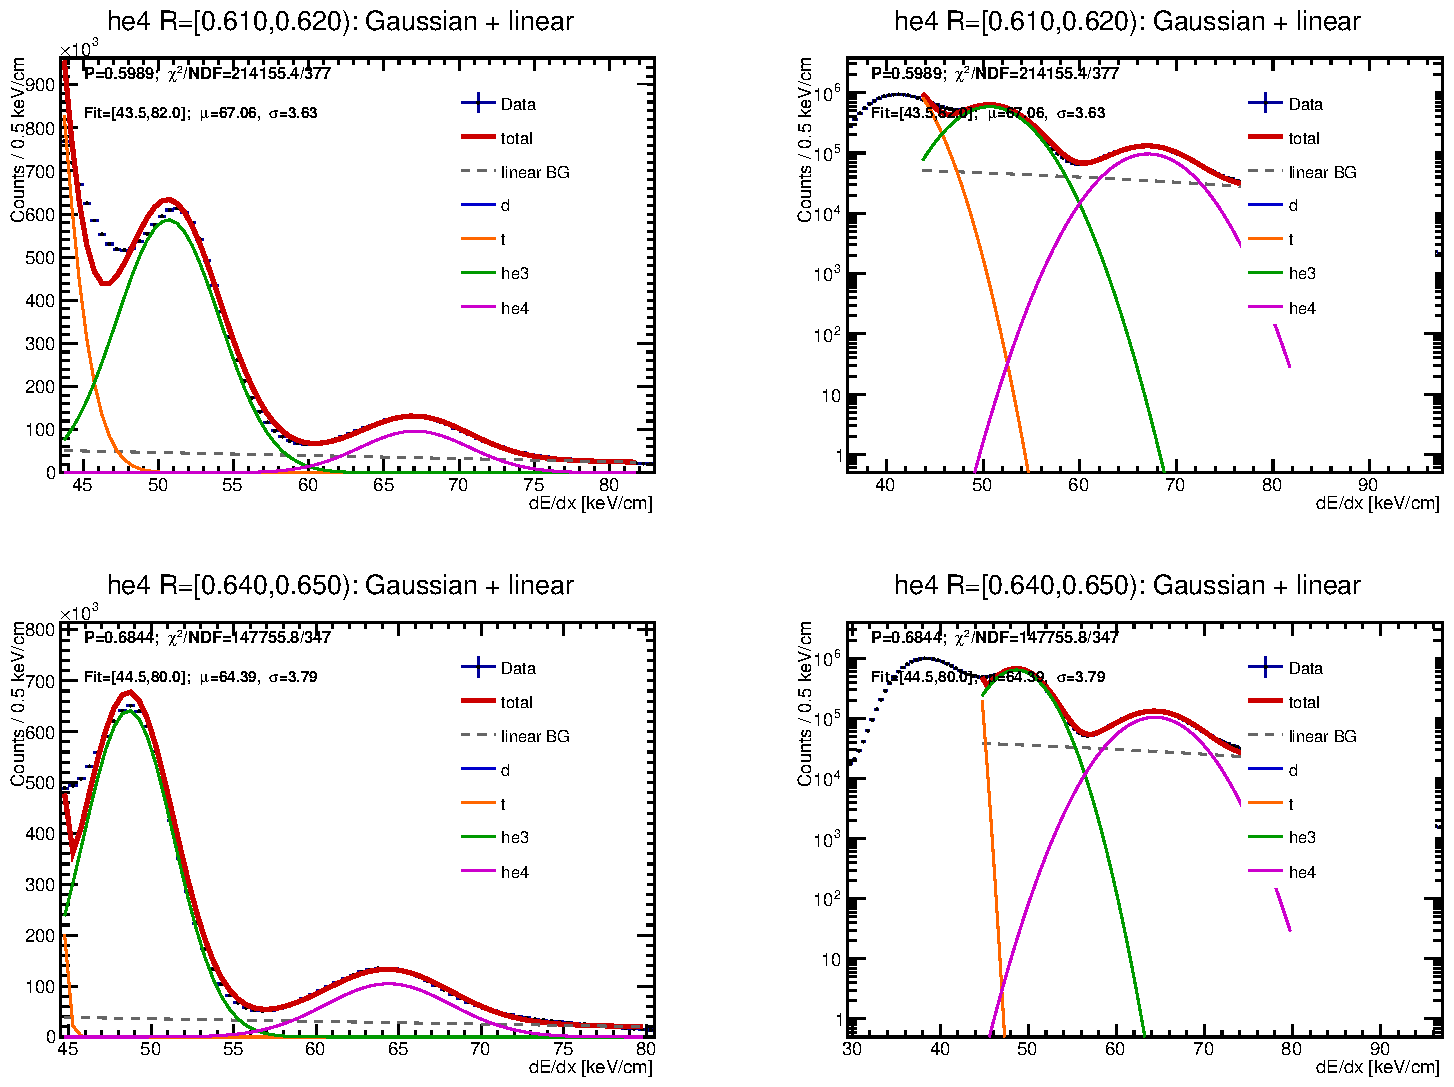
\includegraphics[width=\linewidth,height=.52\textheight,keepaspectratio]{fit_anchors_01_trim.png}\end{center}
\hspace{0pt}{\jpfont 図}\hspace{0pt}5\hspace{0pt}{\jpfont 　上：}\hspace{0pt}[0.61,0.62)\hspace{0pt}{\jpfont 、下：}\hspace{0pt}[0.64,0.65)\hspace{0pt}{\jpfont 。左右は}\hspace{0pt}linear/\allowbreak{}log\hspace{0pt}{\jpfont 表示で、どちらも}\hspace{0pt}Gaussian\hspace{0pt}{\jpfont ＋}\hspace{0pt}linear fit\hspace{0pt}{\jpfont 。}\hspace{0pt}native\hspace{0pt}{\jpfont 中心はそれぞれ}\hspace{0pt}0.615\hspace{0pt}{\jpfont 、}\hspace{0pt}0.645\hspace{0pt}{\jpfont であり、指定}\hspace{0pt}R\hspace{0pt}{\jpfont の無幅分布とは異なる。}\hspace{0pt}

\begin{center}\small\begin{tabular}{lrrr}\toprule
R\hspace{0pt}{\jpfont 区間}\hspace{0pt} & ³He\hspace{0pt}{\jpfont 中心・固定}\hspace{0pt} & ⁴He\hspace{0pt}{\jpfont 中心・自由}\hspace{0pt} & Purity\\\midrule
{}[0.61,0.62) & 50.67 & 67.06 & 59.89\%\\
{}[0.64,0.65) & 48.64 & 64.39 & 68.44\%\\\bottomrule\end{tabular}\end{center}
³He\hspace{0pt}{\jpfont の低側半値を全}\hspace{0pt}fit\hspace{0pt}{\jpfont ・全}\hspace{0pt}GL3\hspace{0pt}{\jpfont 点で含むことを、}\hspace{0pt}fit\hspace{0pt}{\jpfont 後の幅についても検証した。}\hspace{0pt}0.70\hspace{0pt}{\jpfont 以上の}\hspace{0pt}1,300\hspace{0pt}{\jpfont 比較は直前の同じ半値範囲}\hspace{0pt}fit\hspace{0pt}{\jpfont と数値差ゼロ。}\hspace{0pt}


\clearpage
\section*{7. TOF\hspace{0pt}{\jpfont なしの代表}\hspace{0pt}fit\hspace{0pt}{\jpfont ：}\hspace{0pt}d}
TOF m²\hspace{0pt}{\jpfont 選択なしの}\hspace{0pt}ALL\hspace{0pt}{\jpfont 試料。上から}\hspace{0pt}R=[0.80,0.81)\hspace{0pt}{\jpfont 、}\hspace{0pt}[1.20,1.21)\hspace{0pt}{\jpfont 、}\hspace{0pt}[1.60,1.61) GeV/\allowbreak{}c\hspace{0pt}{\jpfont の}\hspace{0pt}3\hspace{0pt}{\jpfont 点を示す。左は}\hspace{0pt}linear\hspace{0pt}{\jpfont 、右は}\hspace{0pt}log\hspace{0pt}{\jpfont 表示。全て}\hspace{0pt}Gaussian\hspace{0pt}{\jpfont 応答＋}\hspace{0pt}linear\hspace{0pt}{\jpfont 背景の保存済み}\hspace{0pt}fit\hspace{0pt}{\jpfont 。}\hspace{0pt}

\begin{center}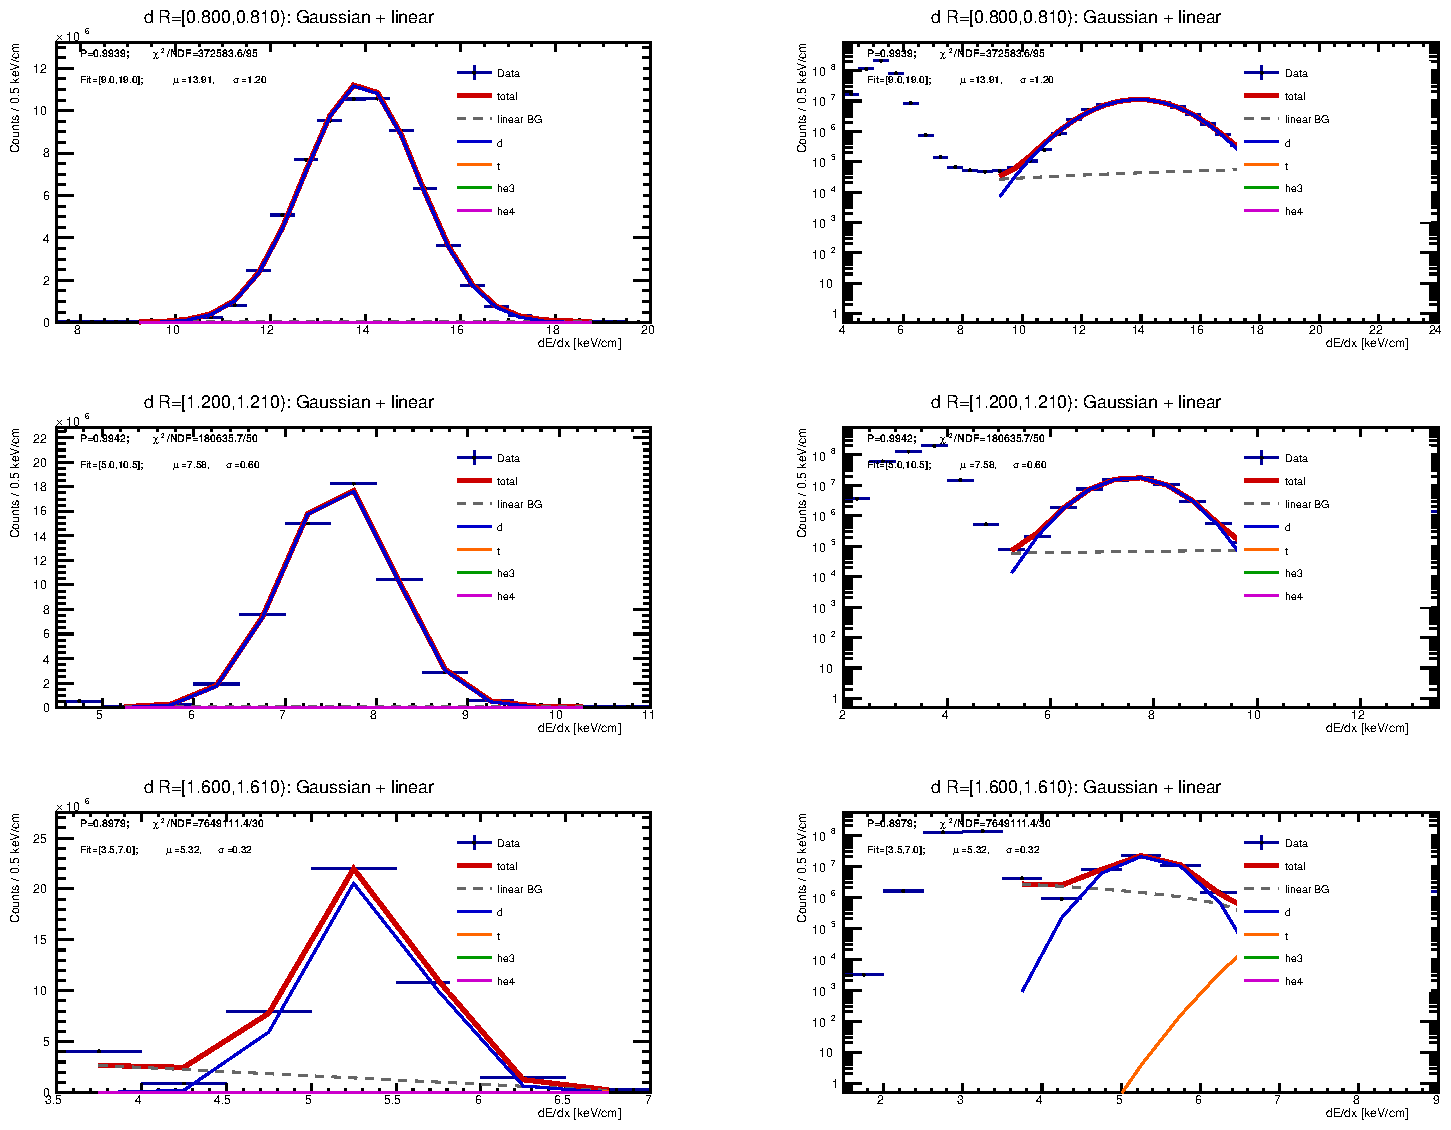
\includegraphics[width=\linewidth,height=.70\textheight,keepaspectratio]{fit_low_d_01_trim.png}\end{center}
\hspace{0pt}{\jpfont 図}\hspace{0pt}6\hspace{0pt}{\jpfont 　}\hspace{0pt}d\hspace{0pt}{\jpfont の異なる}\hspace{0pt}p/\allowbreak{}q\hspace{0pt}{\jpfont における}\hspace{0pt}dE/\allowbreak{}dx fit\hspace{0pt}{\jpfont 。黒：生データ、赤：全成分、灰破線：}\hspace{0pt}linear\hspace{0pt}{\jpfont 背景、色線：核種成分。各段に}\hspace{0pt}R\hspace{0pt}{\jpfont 区間、}\hspace{0pt}Purity\hspace{0pt}{\jpfont 、}\hspace{0pt}χ²/\allowbreak{}NDF\hspace{0pt}{\jpfont 、}\hspace{0pt}fit\hspace{0pt}{\jpfont 範囲、中心と幅を記した。}\hspace{0pt}

\hspace{0pt}{\jpfont 予測曲線は}\hspace{0pt}fit\hspace{0pt}{\jpfont 範囲内だけに表示する。}\hspace{0pt}Purity\hspace{0pt}{\jpfont の分母には他核種と}\hspace{0pt}linear\hspace{0pt}{\jpfont 背景を含む。代表点の追加に伴う再}\hspace{0pt}fit\hspace{0pt}{\jpfont や}\hspace{0pt}Purity\hspace{0pt}{\jpfont 数値の変更はない。}\hspace{0pt}


\clearpage
\section*{8. TOF\hspace{0pt}{\jpfont なしの代表}\hspace{0pt}fit\hspace{0pt}{\jpfont ：}\hspace{0pt}t}
TOF m²\hspace{0pt}{\jpfont 選択なしの}\hspace{0pt}ALL\hspace{0pt}{\jpfont 試料。上から}\hspace{0pt}R=[0.80,0.81)\hspace{0pt}{\jpfont 、}\hspace{0pt}[1.20,1.21)\hspace{0pt}{\jpfont 、}\hspace{0pt}[1.60,1.61) GeV/\allowbreak{}c\hspace{0pt}{\jpfont の}\hspace{0pt}3\hspace{0pt}{\jpfont 点を示す。左は}\hspace{0pt}linear\hspace{0pt}{\jpfont 、右は}\hspace{0pt}log\hspace{0pt}{\jpfont 表示。全て}\hspace{0pt}Gaussian\hspace{0pt}{\jpfont 応答＋}\hspace{0pt}linear\hspace{0pt}{\jpfont 背景の保存済み}\hspace{0pt}fit\hspace{0pt}{\jpfont 。}\hspace{0pt}

\begin{center}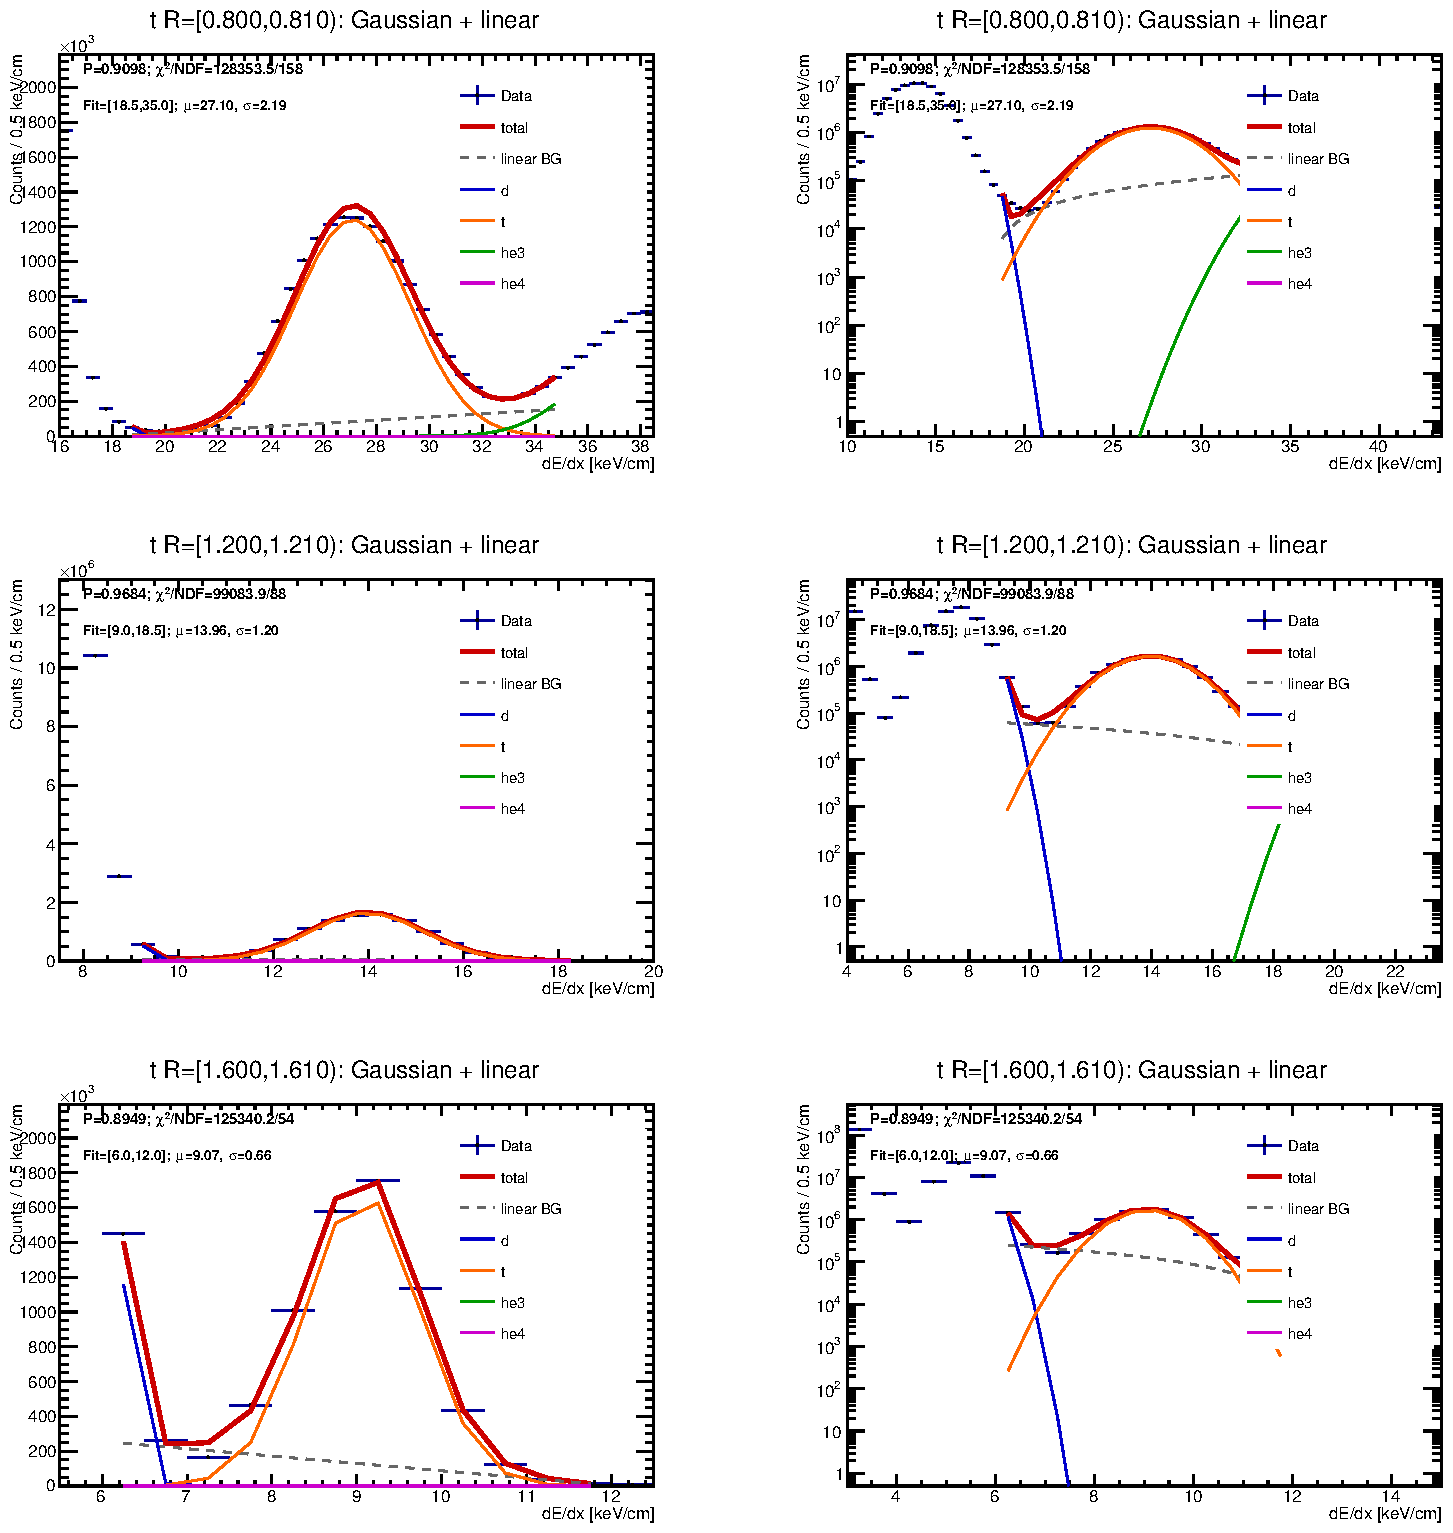
\includegraphics[width=\linewidth,height=.70\textheight,keepaspectratio]{fit_low_t_01_trim.png}\end{center}
\hspace{0pt}{\jpfont 図}\hspace{0pt}7\hspace{0pt}{\jpfont 　}\hspace{0pt}t\hspace{0pt}{\jpfont の異なる}\hspace{0pt}p/\allowbreak{}q\hspace{0pt}{\jpfont における}\hspace{0pt}dE/\allowbreak{}dx fit\hspace{0pt}{\jpfont 。黒：生データ、赤：全成分、灰破線：}\hspace{0pt}linear\hspace{0pt}{\jpfont 背景、色線：核種成分。各段に}\hspace{0pt}R\hspace{0pt}{\jpfont 区間、}\hspace{0pt}Purity\hspace{0pt}{\jpfont 、}\hspace{0pt}χ²/\allowbreak{}NDF\hspace{0pt}{\jpfont 、}\hspace{0pt}fit\hspace{0pt}{\jpfont 範囲、中心と幅を記した。}\hspace{0pt}

\hspace{0pt}{\jpfont 予測曲線は}\hspace{0pt}fit\hspace{0pt}{\jpfont 範囲内だけに表示する。}\hspace{0pt}Purity\hspace{0pt}{\jpfont の分母には他核種と}\hspace{0pt}linear\hspace{0pt}{\jpfont 背景を含む。代表点の追加に伴う再}\hspace{0pt}fit\hspace{0pt}{\jpfont や}\hspace{0pt}Purity\hspace{0pt}{\jpfont 数値の変更はない。}\hspace{0pt}


\clearpage
\section*{9. TOF\hspace{0pt}{\jpfont なしの代表}\hspace{0pt}fit\hspace{0pt}{\jpfont ：}\hspace{0pt}³He}
TOF m²\hspace{0pt}{\jpfont 選択なしの}\hspace{0pt}ALL\hspace{0pt}{\jpfont 試料。上から}\hspace{0pt}R=[0.80,0.81)\hspace{0pt}{\jpfont 、}\hspace{0pt}[1.20,1.21)\hspace{0pt}{\jpfont 、}\hspace{0pt}[1.60,1.61) GeV/\allowbreak{}c\hspace{0pt}{\jpfont の}\hspace{0pt}3\hspace{0pt}{\jpfont 点を示す。左は}\hspace{0pt}linear\hspace{0pt}{\jpfont 、右は}\hspace{0pt}log\hspace{0pt}{\jpfont 表示。全て}\hspace{0pt}Gaussian\hspace{0pt}{\jpfont 応答＋}\hspace{0pt}linear\hspace{0pt}{\jpfont 背景の保存済み}\hspace{0pt}fit\hspace{0pt}{\jpfont 。}\hspace{0pt}

\begin{center}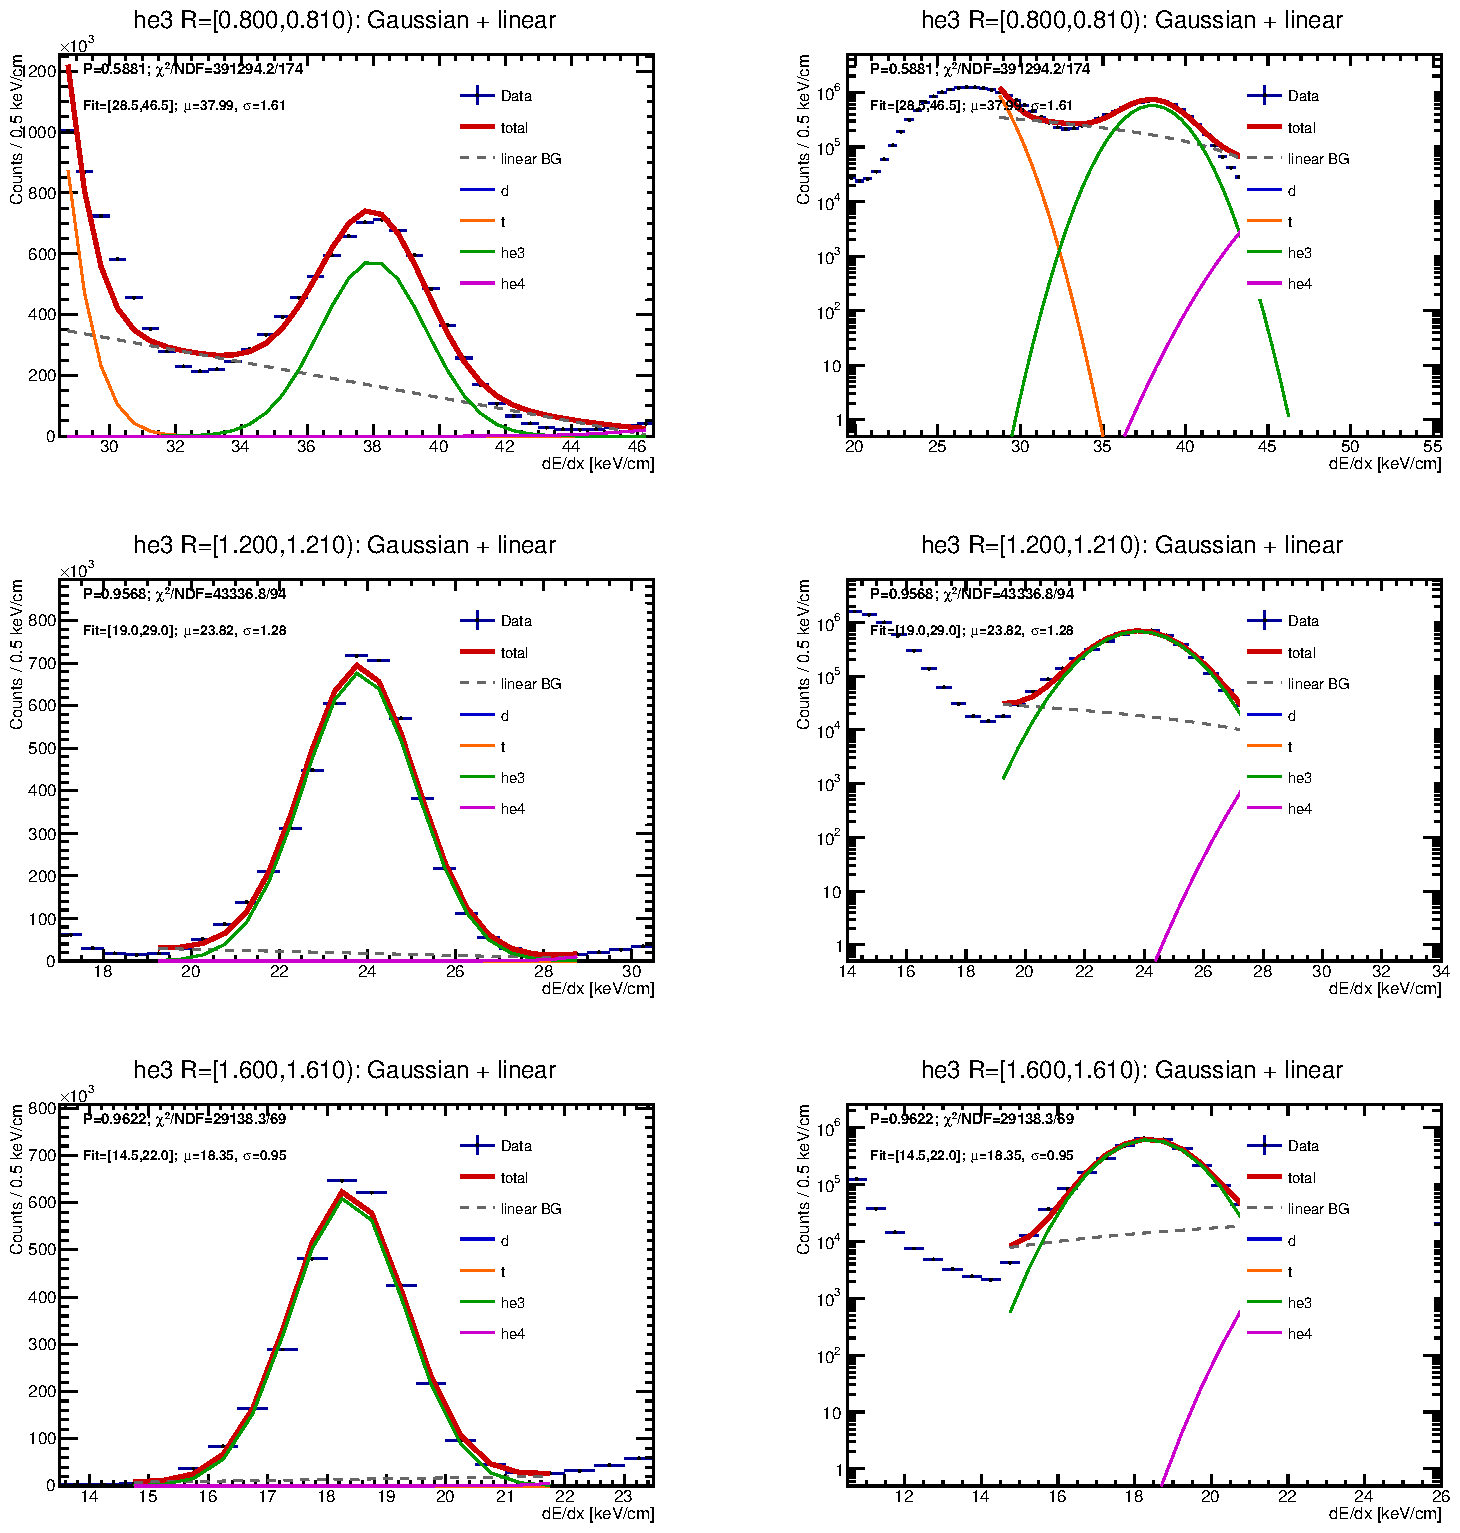
\includegraphics[width=\linewidth,height=.70\textheight,keepaspectratio]{fit_low_he3_01_trim.png}\end{center}
\hspace{0pt}{\jpfont 図}\hspace{0pt}8\hspace{0pt}{\jpfont 　}\hspace{0pt}³He\hspace{0pt}{\jpfont の異なる}\hspace{0pt}p/\allowbreak{}q\hspace{0pt}{\jpfont における}\hspace{0pt}dE/\allowbreak{}dx fit\hspace{0pt}{\jpfont 。黒：生データ、赤：全成分、灰破線：}\hspace{0pt}linear\hspace{0pt}{\jpfont 背景、色線：核種成分。各段に}\hspace{0pt}R\hspace{0pt}{\jpfont 区間、}\hspace{0pt}Purity\hspace{0pt}{\jpfont 、}\hspace{0pt}χ²/\allowbreak{}NDF\hspace{0pt}{\jpfont 、}\hspace{0pt}fit\hspace{0pt}{\jpfont 範囲、中心と幅を記した。}\hspace{0pt}

\hspace{0pt}{\jpfont 予測曲線は}\hspace{0pt}fit\hspace{0pt}{\jpfont 範囲内だけに表示する。}\hspace{0pt}Purity\hspace{0pt}{\jpfont の分母には他核種と}\hspace{0pt}linear\hspace{0pt}{\jpfont 背景を含む。代表点の追加に伴う再}\hspace{0pt}fit\hspace{0pt}{\jpfont や}\hspace{0pt}Purity\hspace{0pt}{\jpfont 数値の変更はない。}\hspace{0pt}


\clearpage
\section*{10. TOF\hspace{0pt}{\jpfont なしの代表}\hspace{0pt}fit\hspace{0pt}{\jpfont ：}\hspace{0pt}⁴He}
TOF m²\hspace{0pt}{\jpfont 選択なしの}\hspace{0pt}ALL\hspace{0pt}{\jpfont 試料。上から}\hspace{0pt}R=[0.80,0.81)\hspace{0pt}{\jpfont 、}\hspace{0pt}[1.20,1.21)\hspace{0pt}{\jpfont 、}\hspace{0pt}[1.60,1.61) GeV/\allowbreak{}c\hspace{0pt}{\jpfont の}\hspace{0pt}3\hspace{0pt}{\jpfont 点を示す。左は}\hspace{0pt}linear\hspace{0pt}{\jpfont 、右は}\hspace{0pt}log\hspace{0pt}{\jpfont 表示。全て}\hspace{0pt}Gaussian\hspace{0pt}{\jpfont 応答＋}\hspace{0pt}linear\hspace{0pt}{\jpfont 背景の保存済み}\hspace{0pt}fit\hspace{0pt}{\jpfont 。}\hspace{0pt}

\begin{center}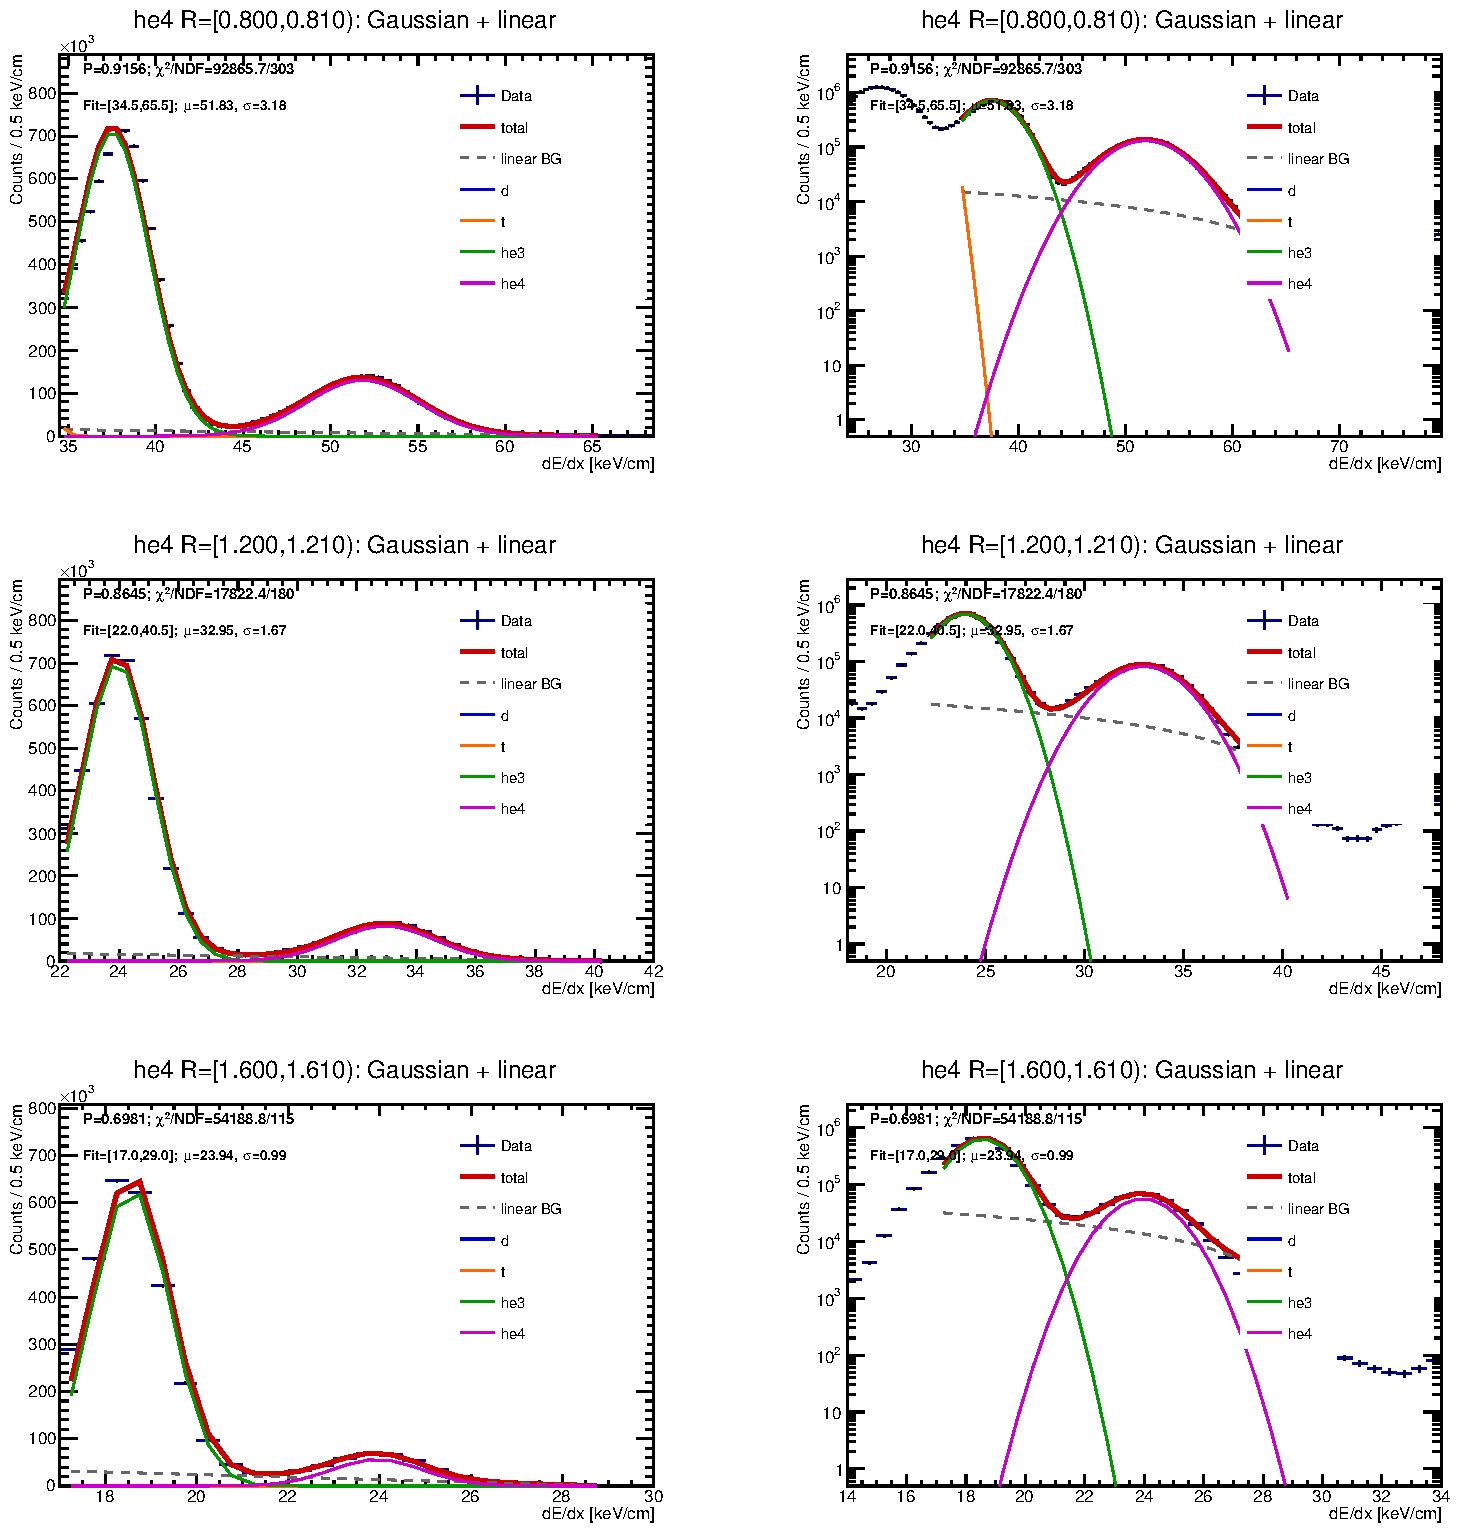
\includegraphics[width=\linewidth,height=.70\textheight,keepaspectratio]{fit_low_he4_01_trim.png}\end{center}
\hspace{0pt}{\jpfont 図}\hspace{0pt}9\hspace{0pt}{\jpfont 　}\hspace{0pt}⁴He\hspace{0pt}{\jpfont の異なる}\hspace{0pt}p/\allowbreak{}q\hspace{0pt}{\jpfont における}\hspace{0pt}dE/\allowbreak{}dx fit\hspace{0pt}{\jpfont 。黒：生データ、赤：全成分、灰破線：}\hspace{0pt}linear\hspace{0pt}{\jpfont 背景、色線：核種成分。各段に}\hspace{0pt}R\hspace{0pt}{\jpfont 区間、}\hspace{0pt}Purity\hspace{0pt}{\jpfont 、}\hspace{0pt}χ²/\allowbreak{}NDF\hspace{0pt}{\jpfont 、}\hspace{0pt}fit\hspace{0pt}{\jpfont 範囲、中心と幅を記した。}\hspace{0pt}

\hspace{0pt}{\jpfont 予測曲線は}\hspace{0pt}fit\hspace{0pt}{\jpfont 範囲内だけに表示する。}\hspace{0pt}Purity\hspace{0pt}{\jpfont の分母には他核種と}\hspace{0pt}linear\hspace{0pt}{\jpfont 背景を含む。代表点の追加に伴う再}\hspace{0pt}fit\hspace{0pt}{\jpfont や}\hspace{0pt}Purity\hspace{0pt}{\jpfont 数値の変更はない。}\hspace{0pt}


\clearpage
\section*{11. TOF\hspace{0pt}{\jpfont 領域の代表}\hspace{0pt}fit\hspace{0pt}{\jpfont ：}\hspace{0pt}d\hspace{0pt}{\jpfont と}\hspace{0pt}t}
\begin{center}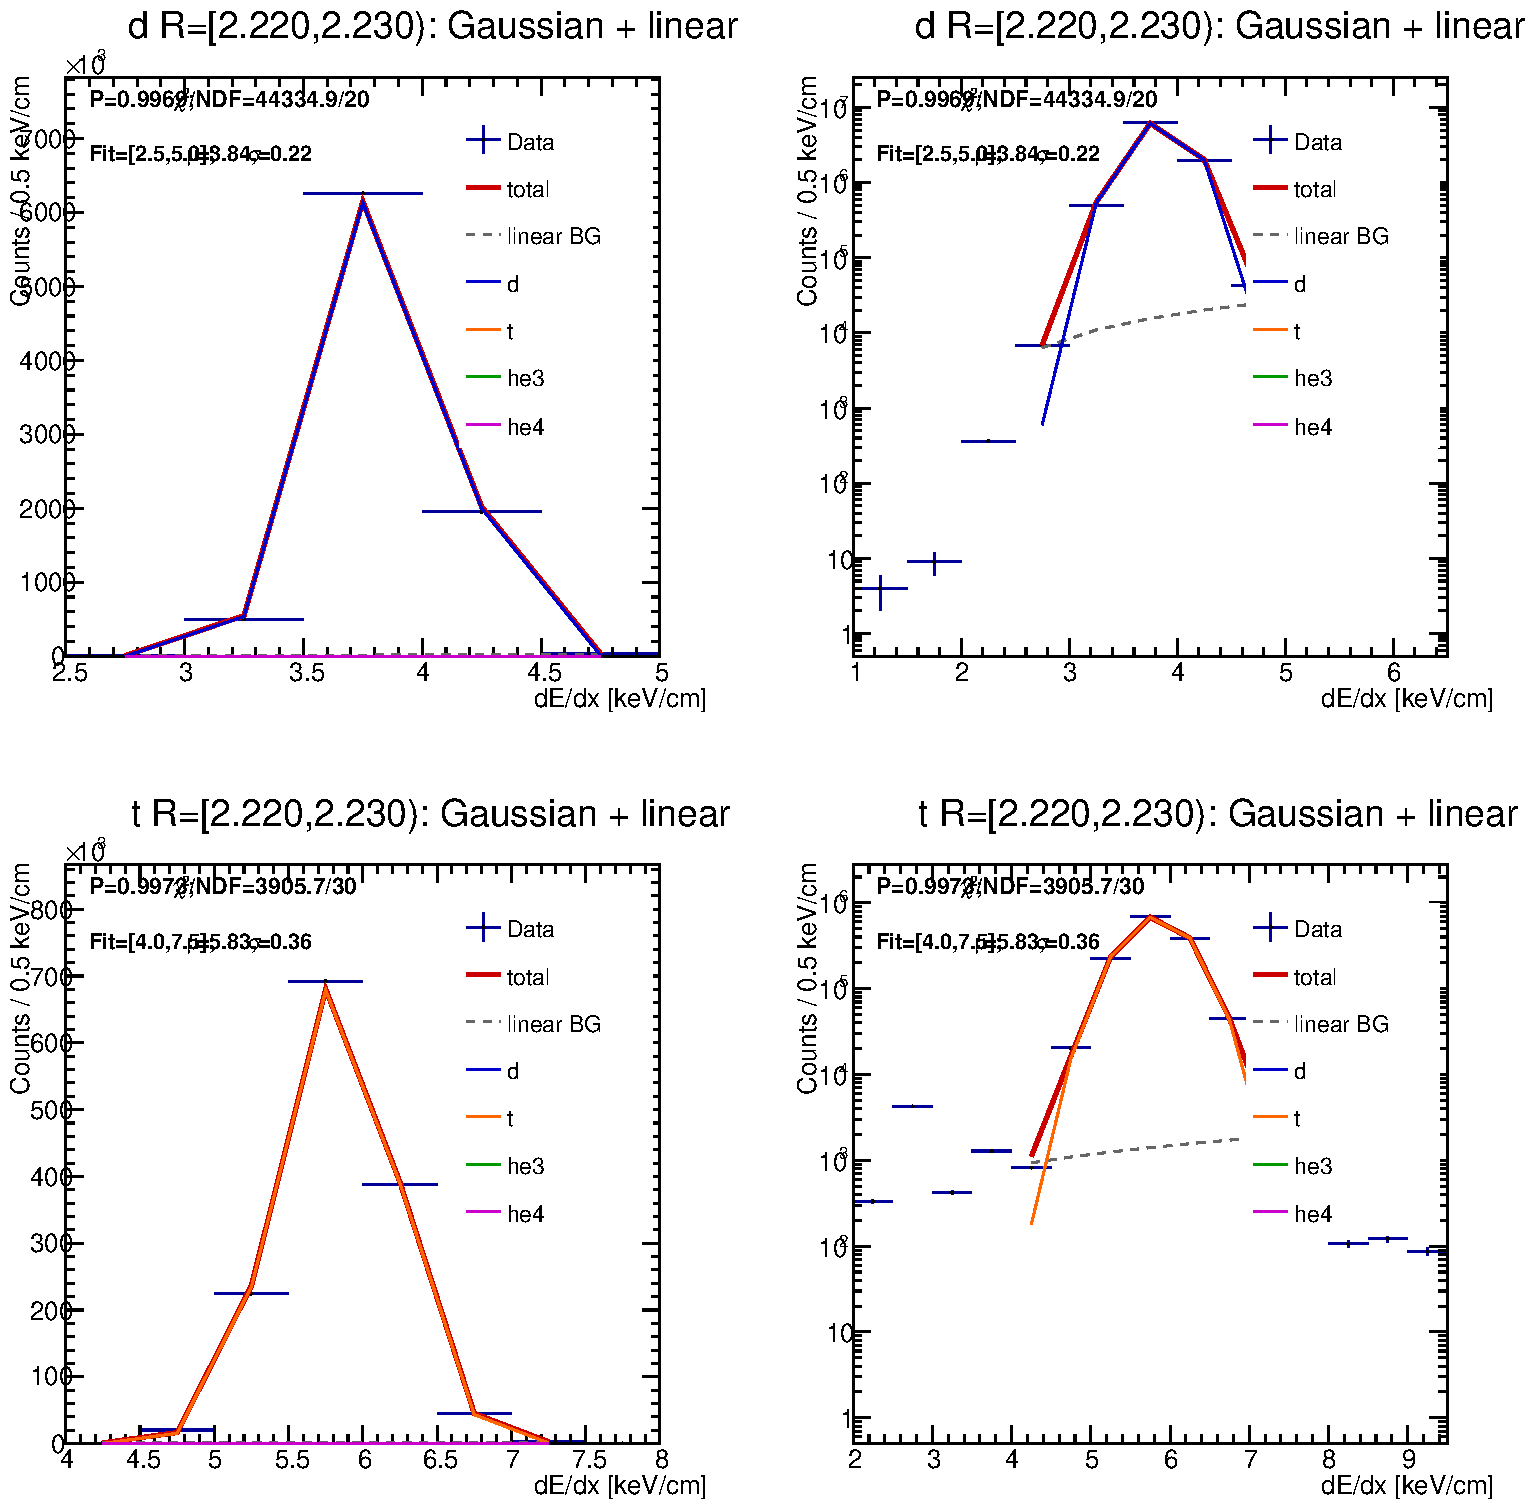
\includegraphics[width=\linewidth,height=.68\textheight,keepaspectratio]{fit_tof_01_trim.png}\end{center}
\hspace{0pt}{\jpfont 図}\hspace{0pt}10\hspace{0pt}{\jpfont 　}\hspace{0pt}R≥2\hspace{0pt}{\jpfont の}\hspace{0pt}TOF\hspace{0pt}{\jpfont 選択試料。既存}\hspace{0pt}m²\hspace{0pt}{\jpfont 窓による選択と}\hspace{0pt}Gaussian\hspace{0pt}{\jpfont ＋}\hspace{0pt}linear\hspace{0pt}{\jpfont の}\hspace{0pt}fit\hspace{0pt}{\jpfont 結果をそのまま使った。低}\hspace{0pt}R\hspace{0pt}{\jpfont の}\hspace{0pt}ALL\hspace{0pt}{\jpfont と高}\hspace{0pt}R\hspace{0pt}{\jpfont の}\hspace{0pt}TOF\hspace{0pt}{\jpfont は試料選択が異なるため、}\hspace{0pt}R=2\hspace{0pt}{\jpfont の境界を明示して}\hspace{0pt}Purity\hspace{0pt}{\jpfont を接続する。}\hspace{0pt}

\hspace{0pt}{\jpfont 高}\hspace{0pt}R\hspace{0pt}{\jpfont の支持判定には、従来の数値収束、応答誤差、収量、核種成分を除いた際の}\hspace{0pt}deviance\hspace{0pt}{\jpfont 差等を用いる。未評価点を補間して延長しない。}\hspace{0pt}


\clearpage
\section*{12. TOF\hspace{0pt}{\jpfont 領域の代表}\hspace{0pt}fit\hspace{0pt}{\jpfont ：}\hspace{0pt}³He\hspace{0pt}{\jpfont と}\hspace{0pt}⁴He}
\begin{center}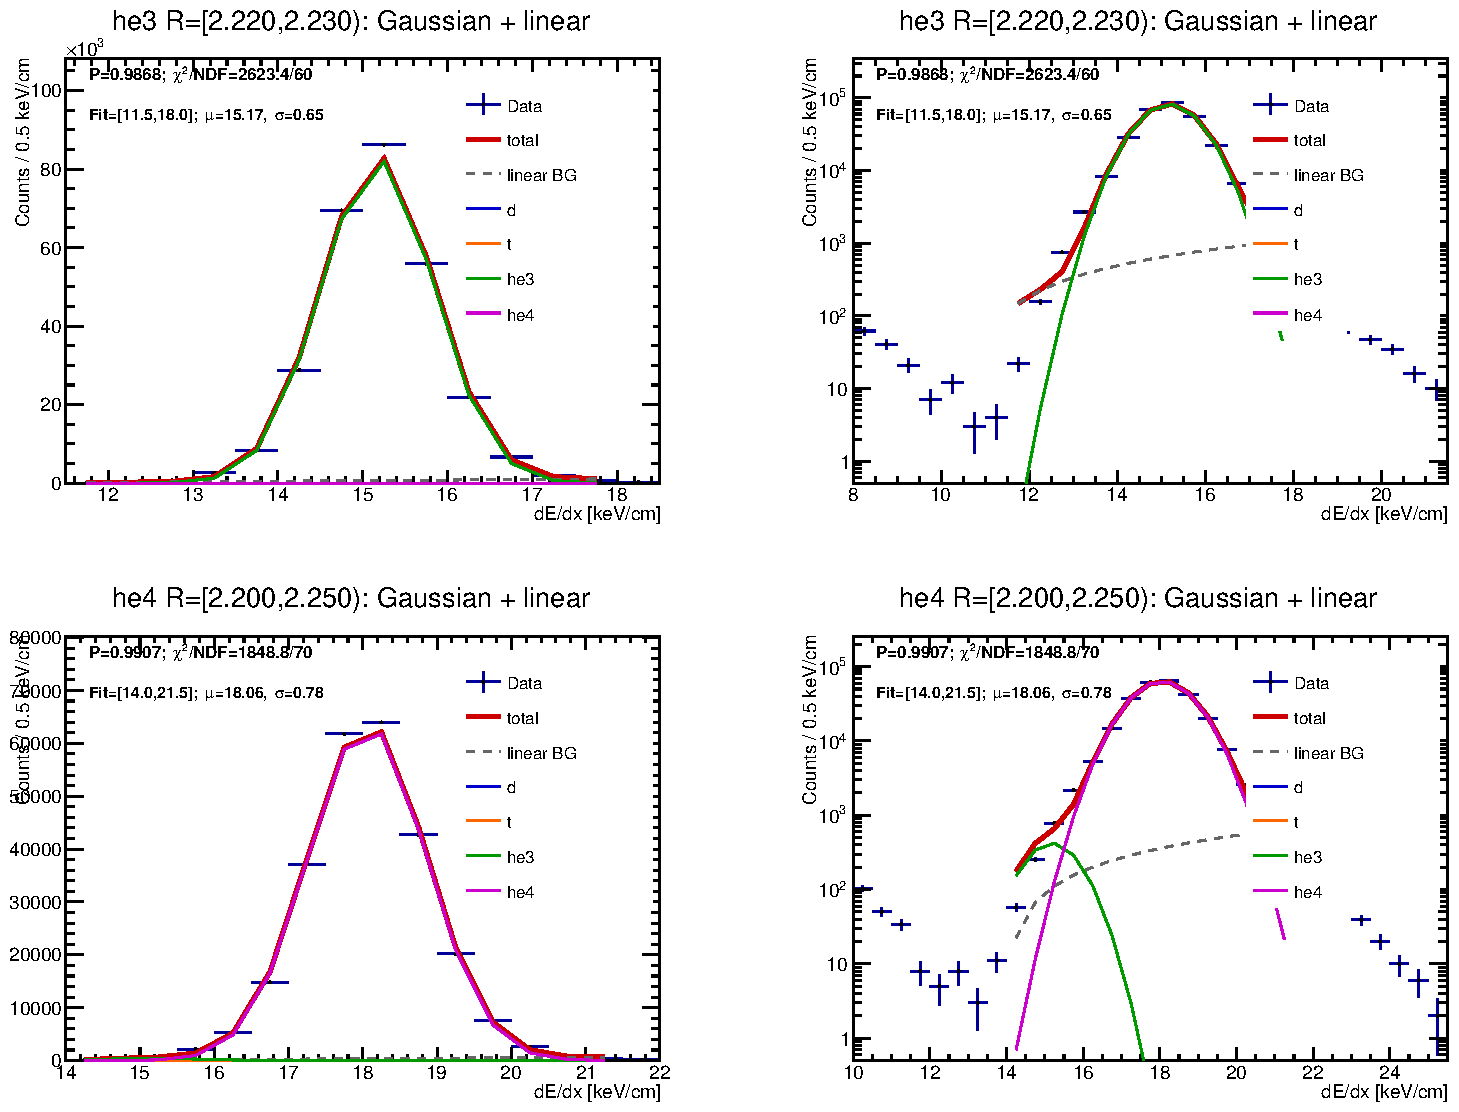
\includegraphics[width=\linewidth,height=.68\textheight,keepaspectratio]{fit_tof_02_trim.png}\end{center}
\hspace{0pt}{\jpfont 図}\hspace{0pt}11\hspace{0pt}{\jpfont 　}\hspace{0pt}³He\hspace{0pt}{\jpfont 、}\hspace{0pt}⁴He\hspace{0pt}{\jpfont の}\hspace{0pt}TOF\hspace{0pt}{\jpfont 領域。}\hspace{0pt}⁴He\hspace{0pt}{\jpfont は}\hspace{0pt}d\hspace{0pt}{\jpfont と}\hspace{0pt}m²\hspace{0pt}{\jpfont が重なるため、}\hspace{0pt}d\hspace{0pt}{\jpfont と同一の}\hspace{0pt}TOF\hspace{0pt}{\jpfont 選択窓を使用する。その後に}\hspace{0pt}dE/\allowbreak{}dx\hspace{0pt}{\jpfont の成分}\hspace{0pt}fit\hspace{0pt}{\jpfont と}\hspace{0pt}PID\hspace{0pt}{\jpfont 積分で}\hspace{0pt}⁴He\hspace{0pt}{\jpfont を評価する。}\hspace{0pt}

TOF m²\hspace{0pt}{\jpfont だけで}\hspace{0pt}d\hspace{0pt}{\jpfont と}\hspace{0pt}⁴He\hspace{0pt}{\jpfont を分離できたと扱わず、両核種の}\hspace{0pt}Gaussian\hspace{0pt}{\jpfont 成分を含めて}\hspace{0pt}Purity\hspace{0pt}{\jpfont を計算する。高}\hspace{0pt}R\hspace{0pt}{\jpfont の元の}\hspace{0pt}fit\hspace{0pt}{\jpfont ・入力}\hspace{0pt}ROOT\hspace{0pt}{\jpfont は変更していない。}\hspace{0pt}


\clearpage
\section*{13. \hspace{0pt}{\jpfont 高}\hspace{0pt}R\hspace{0pt}{\jpfont の}\hspace{0pt}Purity}
\begin{center}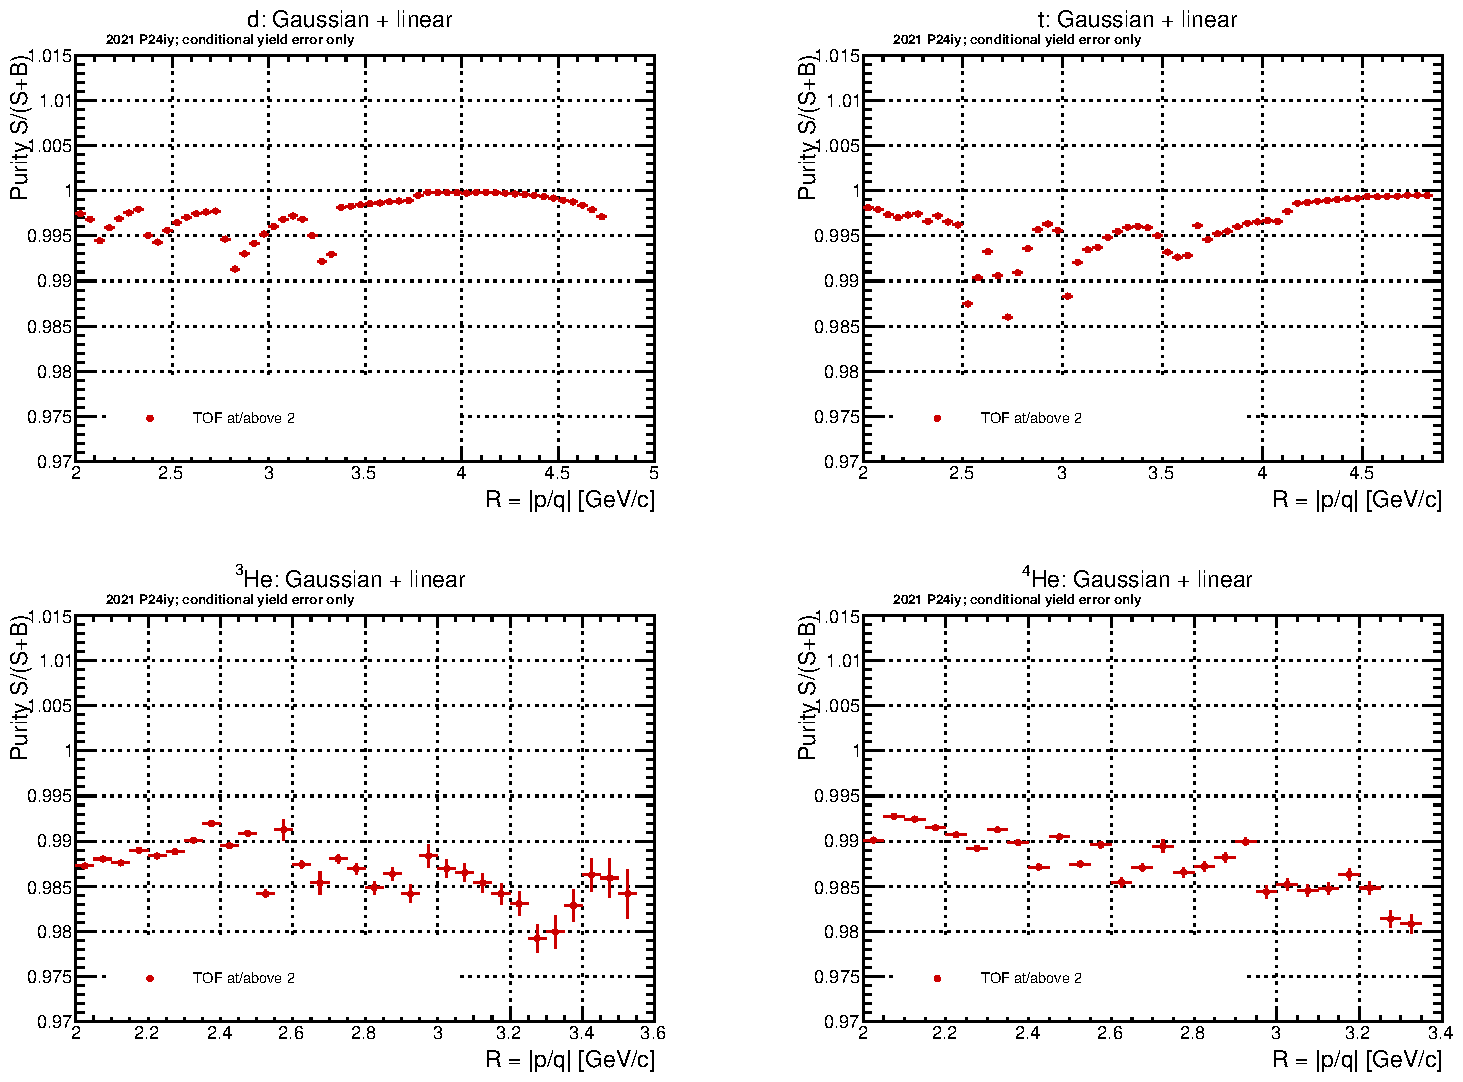
\includegraphics[width=\linewidth,height=.56\textheight,keepaspectratio]{purity_vs_p_over_q_02_trim.png}\end{center}
\hspace{0pt}{\jpfont 図}\hspace{0pt}12\hspace{0pt}{\jpfont 　}\hspace{0pt}Gaussian\hspace{0pt}{\jpfont ＋}\hspace{0pt}linear\hspace{0pt}{\jpfont のみの高}\hspace{0pt}R\hspace{0pt}{\jpfont 表示。誤差棒は条件付き収量誤差で、モデル差の範囲ではない。}\hspace{0pt}

\begin{center}\small\begin{tabular}{lrrr}\toprule
\hspace{0pt}{\jpfont 核種}\hspace{0pt} & \hspace{0pt}{\jpfont 支持点数}\hspace{0pt}/\allowbreak{}\hspace{0pt}{\jpfont 全区間}\hspace{0pt} & \hspace{0pt}{\jpfont 支持点の}\hspace{0pt}R\hspace{0pt}{\jpfont 最小}\hspace{0pt}–\hspace{0pt}{\jpfont 最大}\hspace{0pt} & \hspace{0pt}{\jpfont 最小}\hspace{0pt}Purity\\\midrule
{}d & 55/\allowbreak{}60 & 2.00–4.75 & 99.13\%\\
{}t & 57/\allowbreak{}60 & 2.00–4.85 & 98.60\%\\
{}he3 & 31/\allowbreak{}60 & 2.00–3.55 & 97.92\%\\
{}he4 & 27/\allowbreak{}60 & 2.00–3.35 & 98.08\%\\\bottomrule\end{tabular}\end{center}
\hspace{0pt}{\jpfont 表示範囲は各核種の支持点に合わせた。}\hspace{0pt}d\hspace{0pt}{\jpfont の全体図の横軸は従来の}\hspace{0pt}0.4–5\hspace{0pt}{\jpfont を保持。支持点の最大}\hspace{0pt}R\hspace{0pt}{\jpfont はこの解析での推定可能範囲であり、物理的・統計的な絶対上限の確定ではない。}\hspace{0pt}


\clearpage
\section*{14. \hspace{0pt}{\jpfont 採否、誤差と再現性}\hspace{0pt}}
\hspace{0pt}{\jpfont 最終図の採否は}\hspace{0pt}Gaussian\hspace{0pt}{\jpfont ＋}\hspace{0pt}linear\hspace{0pt}{\jpfont 自身の支持条件だけを使う。以前の複数モデル全体の採否や包絡線を残さず、他モデルの失敗を理由に採用モデルの点を落とさない。一方、}\hspace{0pt}Purity\hspace{0pt}{\jpfont が}\hspace{0pt}50\%\hspace{0pt}{\jpfont 未満の点は隠さず表示する。}\hspace{0pt}

\begin{center}\small\begin{tabular}{lrr}\toprule
\hspace{0pt}{\jpfont 核種}\hspace{0pt} & \hspace{0pt}{\jpfont 集約}\hspace{0pt}R\hspace{0pt}{\jpfont 区間}\hspace{0pt} & Gaussian\hspace{0pt}{\jpfont ＋}\hspace{0pt}linear Purity\\\midrule
{}he3 & 0.65–0.70 & 29.33\%\\
{}he3 & 0.70–0.75 & 34.20\%\\
{}he4 & 1.95–2.00 & 45.04\%\\\bottomrule\end{tabular}\end{center}
⁴He\hspace{0pt}{\jpfont の}\hspace{0pt}R>0.61\hspace{0pt}{\jpfont は適用範囲を表し、全}\hspace{0pt}R\hspace{0pt}{\jpfont で}\hspace{0pt}50\%\hspace{0pt}{\jpfont 以上を保証するものではない。特に}\hspace{0pt}1.95–2.00\hspace{0pt}{\jpfont では}\hspace{0pt}45.04\%\hspace{0pt}{\jpfont が残る。}\hspace{0pt}³He\hspace{0pt}{\jpfont の低}\hspace{0pt}R\hspace{0pt}{\jpfont にも}\hspace{0pt}50\%\hspace{0pt}{\jpfont 未満の区間がある。新しい}\hspace{0pt}veto\hspace{0pt}{\jpfont は自動追加していない。}\hspace{0pt}

\hspace{0pt}{\jpfont 縦誤差は}\hspace{0pt}fit\hspace{0pt}{\jpfont 形状・背景モデルを条件とした収量誤差。集約では各}\hspace{0pt}native\hspace{0pt}{\jpfont 区間の誤差を分母の重みで線形に足した保守的な上限を用いる。}\hspace{0pt}Gaussian/\allowbreak{}linear\hspace{0pt}{\jpfont の選択、応答形状、}\hspace{0pt}³He\hspace{0pt}{\jpfont 参照位置の概数誤差を含む完全な系統誤差ではない。単一モデル表示に変更して誤差棒が小さくなっても、全不確かさが減ったという意味ではない。}\hspace{0pt}

\hspace{0pt}{\jpfont 絶対}\hspace{0pt}χ²/\allowbreak{}NDF\hspace{0pt}{\jpfont が大きい区間もある。支持フラグの通過は}\hspace{0pt}χ²/\allowbreak{}NDF≈1\hspace{0pt}{\jpfont を意味しない。}\hspace{0pt}linear\hspace{0pt}{\jpfont 採用はユーザーによる目視判断と指定を反映したもので、全域での形式的なモデル優越を主張していない。}\hspace{0pt}

\hspace{0pt}{\jpfont 今回の作業は既存}\hspace{0pt}fit\hspace{0pt}{\jpfont の抽出と再描画で、新しい}\hspace{0pt}fit\hspace{0pt}{\jpfont ・イベント解析・本番}\hspace{0pt}PID\hspace{0pt}{\jpfont 反映は行っていない。}\hspace{0pt}364\hspace{0pt}{\jpfont 区間のモデルキー、}\hspace{0pt}ΣS/\allowbreak{}Σtotal\hspace{0pt}{\jpfont 、条件付き誤差と支持フラグを元}\hspace{0pt}JSON\hspace{0pt}{\jpfont へ照合済み。旧}\hspace{0pt}ROOT\hspace{0pt}{\jpfont ・旧図を保持し、入力}\hspace{0pt}SHA\hspace{0pt}{\jpfont と生成物を}\hspace{0pt}manifest\hspace{0pt}{\jpfont に記録する。}\hspace{0pt}

\hspace{0pt}{\jpfont 再現ファイル：同梱}\hspace{0pt}settings.yaml\hspace{0pt}{\jpfont 、}\hspace{0pt}purity.tsv\hspace{0pt}{\jpfont 、}\hspace{0pt}summary.json\hspace{0pt}{\jpfont 、}\hspace{0pt}coefficients.json\hspace{0pt}{\jpfont 、}\hspace{0pt}examples.tsv\hspace{0pt}{\jpfont 。元は}\hspace{0pt}candidate\_\allowbreak{}summary.json\hspace{0pt}{\jpfont と}\hspace{0pt}he4\_\allowbreak{}r061\_\allowbreak{}001/\allowbreak{}summary.json\hspace{0pt}{\jpfont 。再現ツールは同梱}\hspace{0pt}source/\allowbreak{}\hspace{0pt}{\jpfont に保存。}\hspace{0pt}

mainconf\hspace{0pt}{\jpfont ：}\hspace{0pt}main\_\allowbreak{}auau3p85\_\allowbreak{}anaFemtoLambda\_\allowbreak{}4He\_\allowbreak{}KFParticle.yaml\hspace{0pt}{\jpfont 。描画は}\hspace{0pt}script/\allowbreak{}singularity\_\allowbreak{}root\_\allowbreak{}batch.sh\hspace{0pt}{\jpfont 経由の}\hspace{0pt}STAR SL24y /\allowbreak{} ROOT5\hspace{0pt}{\jpfont 。ローカル}\hspace{0pt}study\hspace{0pt}{\jpfont のため新規}\hspace{0pt}jobid/\allowbreak{}configlog\hspace{0pt}{\jpfont なし。}\hspace{0pt}PDF\hspace{0pt}{\jpfont 組版は}\hspace{0pt}XeLaTeX\hspace{0pt}{\jpfont 。図の}\hspace{0pt}vector PDF\hspace{0pt}{\jpfont と}\hspace{0pt}200 dpi\hspace{0pt}{\jpfont 画像を両方保存。}\hspace{0pt}job\hspace{0pt}{\jpfont 投入・}\hspace{0pt}hadd\hspace{0pt}{\jpfont ・}\hspace{0pt}commit/\allowbreak{}push\hspace{0pt}{\jpfont なし。}\hspace{0pt}


\end{document}
